\documentclass[10pt, a4paper]{article}

\usepackage{a4wide}
\usepackage{listings}
\usepackage{comment}
\usepackage{amsmath}
\usepackage{graphicx}
\usepackage{amssymb}
\usepackage{url}
\usepackage{hyperref}

\hypersetup{
  colorlinks = true, % colours links instead of ugly boxes
  urlcolor = blue, %  colour for external hyperlinks
  linkcolor = black, % colour of internal links
  citecolor = black, % colour of citations
  pdftitle = {A Survey of Symbolic Execution Techniques},
  pdfauthor= {Roberto Baldoni, Emilio Coppa, \\ Daniele Cono D'Elia, Camil Demetrescu, Irene Finocchi}
}	

\setlength{\parindent}{0pt}

\title{A Survey of Symbolic Execution Techniques}

\author{
Roberto Baldoni, Emilio Coppa, \\ 
Daniele Cono D'Elia, Camil Demetrescu, Irene Finocchi\\
SEASON Lab  \\
\url{season-lab.github.io} \\
Sapienza University of Rome  \\
}

%\date{}

\begin{document}

\maketitle
%\setcounter{tocdepth}{3}
\tableofcontents

\newpage

% !TEX root = main.tex

\epigraph{\textit{``Sometimes you can't see how important something is in its moment, even if it seems kind of important. This is probably one of those times.''}}{(Cyber Grand Challenge highlights from DEF CON 24, August 6, 2016)}

\section{Introduction}
\label{se:intro}

Symbolic execution is a popular program analysis technique first introduced in the mid '70s in the context of software testing to check if a certain property can be violated by a program~\cite{K-ICRS75,SELECT-ICRS75,K-CACM76,H-TSE77}. Aspects of interest could be that no division by zero is ever performed, no {\tt NULL} pointer is ever dereferenced, no backdoor exists that can bypass authentication, etc. While in general there is no automated way to decide some properties (e.g., the target of an indirect jump), heuristics and approximate analyses can prove useful in practice in a variety of settings, including mission-critical and security applications.

%While in general there is no automated way to decide some properties (think, e.g., of the halting problem), decidable approximations often exist (e.g., ``does a program always terminate within a certain amount of time?''). Such approximations can prove useful in practice in a variety of settings, including mission-critical and security applications.

In a concrete execution, a program is run on a specific input and a single control flow path is explored. Hence, in most cases concrete executions can only underapproximate the analysis of the property of interest. In contrast, symbolic execution can simultaneously explore multiple paths that a program could take under different inputs. This paves the road to sound analyses that can yield strong guarantees on the checked property. 
%\mynote{I: a cosa serve ridirlo? Abbiamo gia' fatto esempi di proprieta' che possono essere verificate}Symbolic execution may answer useful questions on concrete programs like: ``does function {\tt foo(x)} always return a positive value for any possible value of {\tt x}?'' 
The key idea is to allow a program to take on {\em symbolic} -- rather than concrete -- input values. Execution is performed by a {\em symbolic execution engine}, which maintains for each explored control flow path: (i) a first-order Boolean {\em formula} that describes the conditions satisfied by the branches taken along that path, and (ii) a {\em symbolic memory store} that maps variables to symbolic expressions or values. Branch execution updates the formula, while assignments update the symbolic store. A {\em model checker}, typically based on a {\em satisfiability modulo theories} (SMT) solver~\cite{HandbookOfSAT2009}, is eventually used to verify if there are any violations of the property along each explored path and if the path itself is realizable, i.e., if its formula can be satisfied by some assignment of concrete values to the program's symbolic arguments.

%Variables and control flow paths are associated with expressions and constraints in terms of those symbols during a symbolic execution of the program, and constraints are eventually solved via SMT (satisfiability modulo theories) solvers.

Symbolic execution techniques have been brought to the attention of a heterogenous audience since DARPA announced in 2013 the Cyber Grand Challenge, a two-year competition seeking to create automatic systems for vulnerability detection, exploitation, and patching in near real-time~\cite{ANGR-SSP16}.

More remarkably, symbolic execution tools have been running 24/7 in the testing process of many Microsoft applications since 2008, revealing for instance nearly one third of the bugs discovered during the development of Windows 7, which were missed by other static program analyses and blackbox testing techniques~\cite{SAGE-QUEUE12}.

In this article, we survey the main aspects of symbolic execution and discuss its extensive usage in software testing and computer security applications, where software vulnerabilities can be found by symbolically executing programs at the level of either source or binary code. We start with a simple example that highlights many of the fundamental issues addressed in the remainder of the article.

% --------------------------------------------------------------------------------------------------------------------
\subsection{A Warm-up Example}
\label{symbolic-execution-example}

Consider the C code of Figure~\ref{fig:example-1} and assume that our goal is to determine which inputs make the  {\tt assert} at line 8 of function \texttt{foobar} fail. Since each input parameter can take as many as $2^{32}$ distinct integer values, the approach of running concretely function \texttt{foobar} on randomly generated inputs will unlikely pick up exactly the assert-failing inputs.
%Techniques such as random testing could generate bottomless input tests for this function. 
%However, it is unlikely that exactly the assert-failing inputs would be randomly picked up\mynote{Fuzzing?}. 
By evaluating the code using symbols for its inputs, instead of concrete values, symbolic execution overcomes this limitation and makes it possible to reason on {\em classes of inputs}, rather than single input values. 

\begin{figure}[t]
\begin{center}
\begin{tabular}{c}
\begin{lstlisting}[basicstyle=\ttfamily\small]
1.  void foobar(int a, int b) {
2.     int x = 1, y = 0;
3.     if (a != 0) {
4.        y = 3+x;
5.        if (b == 0)
6.           x = 2*(a+b);
7.     }
8.     assert(x-y != 0);
9.  }
\end{lstlisting}
\end{tabular}
\end{center}
\caption{Warm-up example: which values of \texttt{a} and \texttt{b} make the \texttt{assert} fail?}
\label{fig:example-1}
\end{figure}

In more detail, every value that cannot be determined by a static analysis of the code, such as an actual parameter of a function or the result of a system call that reads data from a stream, is represented by a symbol $\alpha_i$. At any time, the symbolic execution engine maintains a state $(stmt,~\sigma,~\pi)$ where:

\begin{itemize}

\item $stmt$ is the next statement to evaluate. For the time being, we assume that $stmt$ can be an assignment, a conditional branch, or a jump (more complex constructs such as function calls and loops will be discussed in  Section~\ref{se:executors} and Section~\ref{se:loops}, respectively).

%\item $\sigma$ is a {\em symbolic store} that associates program variables with expressions over \mynote{[D] $\alpha_i$ also concrete?} concrete and symbolic values $\alpha_i$.

\item $\sigma$ is a {\em symbolic store} that associates program variables with either expressions over concrete values or symbolic values $\alpha_i$.

\item $\pi$ denotes the {\em path constraints}, i.e., is a formula that expresses a set of assumptions on the symbols $\alpha_i$ due to branches taken in the execution to reach $stmt$. At the beginning of the analysis, $\pi=true$.

\end{itemize}

\noindent Depending on $stmt$, the symbolic engine changes the state as follows:

\begin{itemize}
  \item The evaluation of an assignment $x=e$ updates the symbolic store $\sigma$ by associating $x$ with a new symbolic expression $e_s$. We denote this association with $x\mapsto e_s$, where $e_s$ is obtained by evaluating $e$ in the context of the current execution state and  can be any expression involving unary or binary operators over symbols and concrete values.
  
%   $\alpha_i = e$: when an expression $e$ is assigned to a symbol $\alpha_i$, $pc$ is extended by adding a constraint on $\alpha_i$:
%    \[ pc \gets pc \wedge \alpha_i = e\]
%  where $e$ can be any expression, involving unary or binary operators, over symbols and constants.

  \item The evaluation of a conditional branch ${\tt if}~e~{\tt then}~s_{true}~{\tt else}~s_{false}$ affects the path constraints $\pi$. The symbolic execution is forked by creating two execution states with path constraints $\pi_{true}$ and $\pi_{false}$, respectively, which correspond to the two branches: $\pi_{true}=\pi \wedge e_s$ and $\pi_{false}=\pi \wedge \neg e_s$, where $e_s$ is a symbolic expression obtained by evaluating $e$. 
%        \[ (s_{true}, pc_{true}) \text{ where } pc_{true} = pc \wedge e \]
%        \[ (s_{false}, pc_{false}) \text{ where } pc_{false} = pc \wedge \neg e \]
    Symbolic execution independently proceeds on both states.

  \item The evaluation of a jump {\tt goto} $s$ updates the execution state by advancing the symbolic execution to statement $s$. 
\end{itemize}

%\subsection{Example}
%\label{symbolic-execution-example}

%\begin{figure}[t]
%  \centering
%  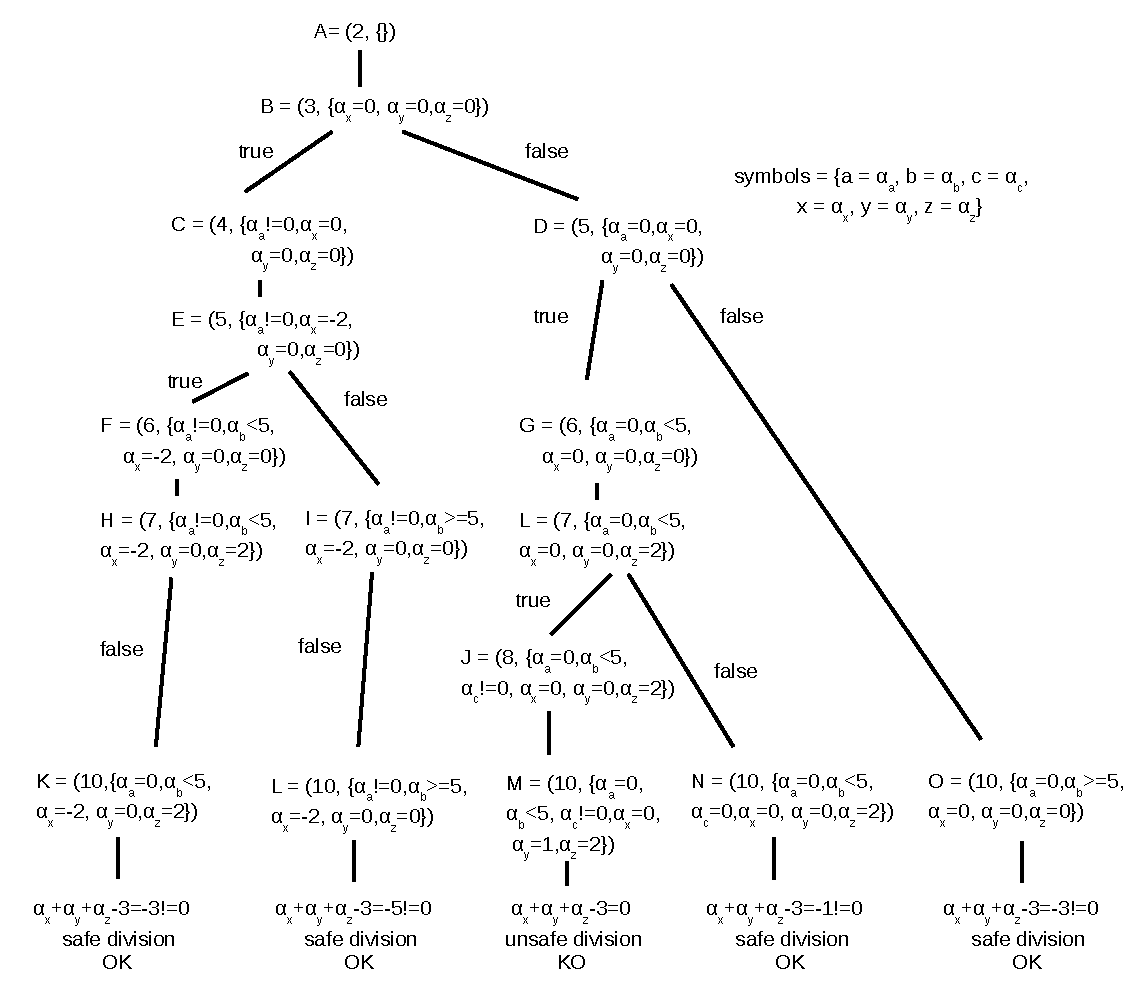
\includegraphics[width=1.0\columnwidth]{images/example} 
%  \caption{Symbolic execution tree of the function {\tt foobar}. Each execution state is labeled with an alphabet letter. Side effects on execution states are highlighted in gray. Leaves are evaluated against division by zero error. For the sake of presentation the conjunction of constraints is shown as a list of constraints. }
%  \label{fig:example-symbolic-execution}
%\end{figure}

\begin{figure}[t]
  \centering
  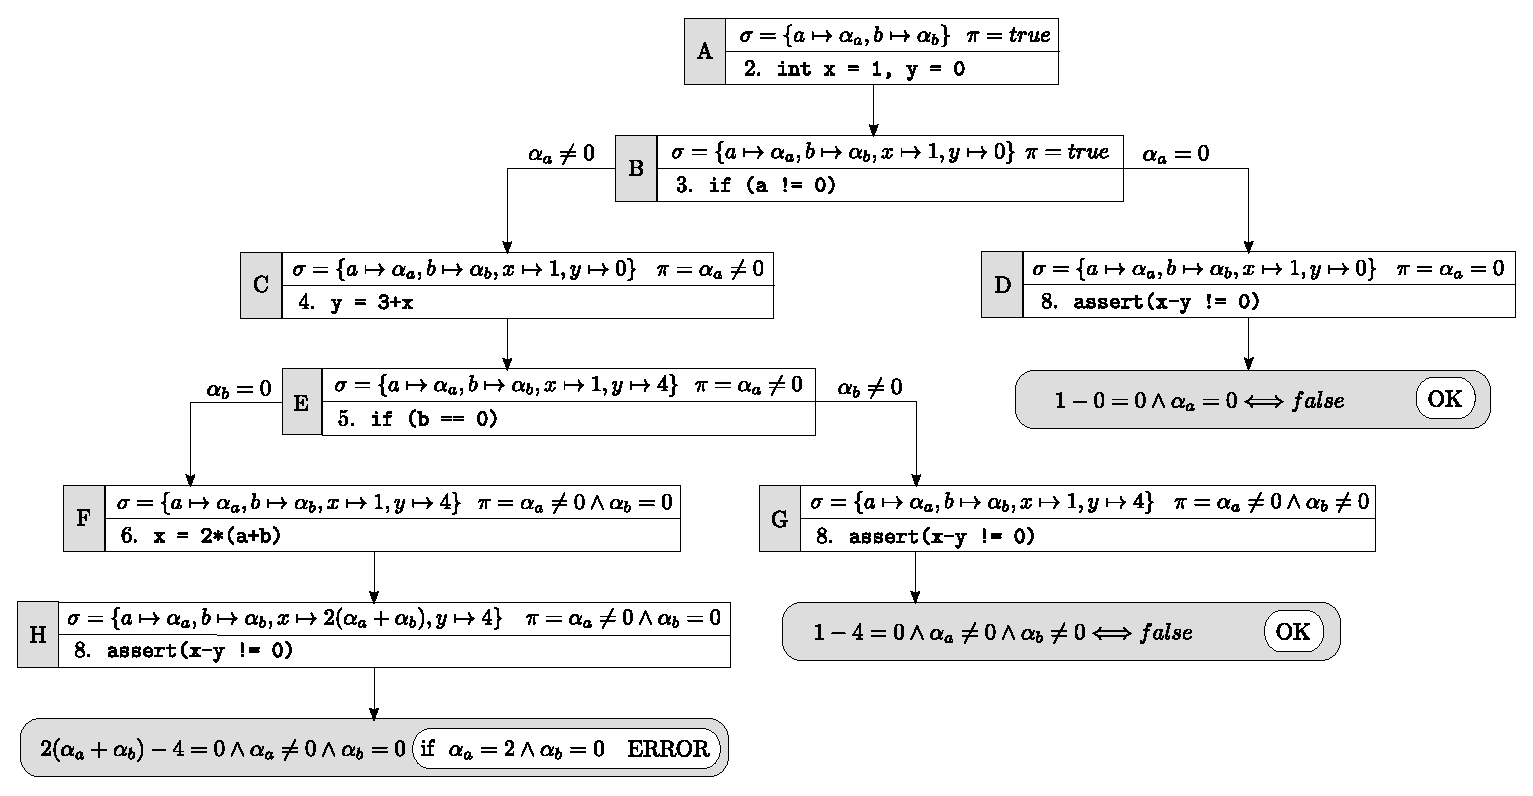
\includegraphics[width=1.0\columnwidth]{images/execution-tree.eps} 
  \caption{Symbolic execution tree of function {\tt foobar} given in Figure~\ref{fig:example-1}. Each execution state, labeled with an upper case letter, shows the statement to be executed, the symbolic store $\sigma$, and the path constraints $\pi$. Leaves are evaluated against the condition in the {\tt assert} statement. }
%For the sake of presentation the conjunction of constraints is shown as a list of constraints. }
  \label{fig:example-symbolic-execution}
\end{figure}

\noindent A symbolic execution of function {\tt foobar} is shown in Figure~\ref{fig:example-symbolic-execution}. Initially (execution state $A$) the path constraints are {\tt true} and input arguments {\tt a} and {\tt b} are associated with symbolic values. 
After initializing local variables {\tt x} and {\tt y} at line 2, the symbolic store is updated by associating {\tt x} and {\tt y} with concrete values 1 and 0, respectively (execution state $B$). Line 3 contains a conditional branch and the execution is forked: depending on the branch taken, a different statement is evaluated next and different assumptions are made on symbol $\alpha_a$ (execution states $C$ and $D$, respectively). In the branch where $\alpha_a\neq 0$, variable {\tt y} is assigned with ${\tt x}+3$, obtaining $y\mapsto 4$ in state $E$ because $x\mapsto 1$ in state $C$. In general, arithmetic expression evaluation simply manipulates the symbolic values.
After expanding every execution state until the {\tt assert} at line 8 is reached on all branches, we can check which input values for parameters {\tt a} and {\tt b} can make the {\tt assert} fail. By analyzing execution states $\{D,G,H\}$, we can conclude that only $H$ can make {\tt x-y = 0} true. The path constraints for $H$ at this point implicitly define the set of inputs that are unsafe for {\tt foobar}. 
In particular, any input values such that:
 \[ 2(\alpha_a+\alpha_b)-4 = 0 \wedge \alpha_a \neq 0 \wedge \alpha_b = 0 \]
will make {\tt assert} fail. An instance of unsafe input parameters can be eventually determined by invoking a {\em model checker}~\cite{HandbookOfSAT2009} to solve the path constraints, which in this example would yield $a = 2$ and $b = 0$. 

%Notice\mynote{Say earlier?} that a constraint solver is also needed when evaluating the satisfiability of branch conditions.

% --------------------------------------------------------------------------------------------------------------------
\subsection{Challenges in Symbolic Execution}
\label{example-discussion}

In the example discussed in Section~\ref{symbolic-execution-example} symbolic execution can identify {\em all} the possible unsafe inputs that make the {\tt assert} fail. This is achieved through an exhaustive exploration of the possible execution states. From a theoretical perspective, exhaustive symbolic execution provides a {\em sound} and {\em complete} methodology for any decidable analysis. Soundness prevents false negatives, i.e., all possible unsafe inputs are guaranteed to be found, while completeness prevents false positives, i.e.,  input values deemed as unsafe are actually unsafe. As we will discuss later on, exhaustive symbolic execution is unlikely to scale beyond small applications. Hence, in practice we often settle for less ambitious goals, e.g., by trading soundness for performance.

Challenges that symbolic execution has to face when processing real-world code can be significantly more complex than those illustrated in our warm-up example. Several observations and questions naturally arise:

\begin{itemize}[itemsep=2mm]

\item \noindent {\em Memory}: how does the symbolic engine handle pointers, arrays, or other complex objects? Any arbitrarily complex object can be regarded as an array of bytes and each byte associated with a distinct symbol. However, when possible, exploiting structural properties of the data may be more convenient: for instance, relational bounds on the class fields in object-oriented languages could be used for refining the search performed by symbolic execution.
%\vspace{1mm}

  \item {\em Environment}: how does the symbolic engine handle interactions with the environment?
  Real-world applications constantly interact with the environment (e.g., the file system or the network) through libraries and system calls. These interactions may cause side-effects
(such as the creation of a file) that could later affect the execution and must be therefore taken into account. Evaluating any possible interaction outcome is generally unfeasible: it could generate a large number of execution states, of which only a small number can actually happen in a non-symbolic scenario. A typical strategy is to consider popular library and system routines and create models that can help the symbolic engine analyze only significant outcomes.
%\vspace{1mm}

  \item {\em Loops}: how does the symbolic engine handle loops?
%A loop\mynote{IF: rimuoverei la prima frase, perche' va detto?} can be encoded using conditional branches and {\tt goto} statements, which is typical  when compiling high-level languages to an intermediate representation or native code. 
Choosing the number of loop iterations to analyze is especially critical when this number cannot be determined in advance (e.g., depends on an input parameter). The naive approach of unrolling iterations for every valid bound would result in a prohibitively large number of states. Typical solutions are to compute an underapproximation of the analysis by limiting the number of iterations to some value $k$, thus trading speed for soundness. Other approaches infer loop invariants through static analysis  and use them to merge equivalent states. % \mynote{i.e. or e.g.?}  (e.g., when differences are not observable from outside the loop body).
%\vspace{1mm}

  \item {\em State space explosion and path selection}: how does symbolic execution deal with path explosion?
Language constructs such as loops might exponentially increase the number of execution states. It is thus unlikely that a symbolic execution engine can exhaustively explore all the possible states within a reasonable amount of time. In practice, heuristics are used to guide exploration and prioritize certain states first (e.g., to maximize code coverage). In addition, symbolic engines can implement efficient mechanisms for evaluating multiple states in parallel without running out of resources.
  %In practice, several heuristics must be exploited to prioritize evaluation of some states, hoping to still be able to spot interesting things. Moreover, the symbolic execution engine should include efficient mechanism for efficiently evaluating in parallel different execution states without running out of computational resources.
%\vspace{1mm}

  \item {\em Constraint solver}: what can a constraint solver do in practice?
  %{\em What is a constraint solver in practice}? \\
 Constraint solvers suffer from a number of limitations. They can typically handle complex constraints in a reasonable amount of time only if they are made of linear expressions over their constituents. Symbolic execution engines normally implement a number of optimizations to make queries as much {\em solver-friendly} as possible, for instance by splitting queries into independent components to be processed separately or by performing algebraic simplifications.
%\vspace{1mm}

  \item {\em Binary code}: what issues can arise when symbolically executing binary code?
  %what are the disadvantages of symbolically executing binary code?
 While the warm-up example of Section~\ref{symbolic-execution-example} is written in C, in several scenarios binary code is the only available representation of a program. However, having the source code of an application can make symbolic execution significantly easier, as it can exploit high-level properties (e.g., object shapes) that can be inferred statically by analyzing the source code.
  %(e.g., the maximum size of a buffer or the number of iterations for a loop).
   
\end{itemize}
%Depending on the specific application context of symbolic execution

\noindent Depending on the specific context in which symbolic execution is used, different choices and assumptions are made to address the questions highlighted above. Although these choices typically affect soundness or completeness, in several scenarios a partial exploration of the space of possible execution states may be sufficient to achieve the goal\mynote{Better example?} (e.g., identifying a crashing input for an application) within a limited time budget.

%different choices and assumptions are made to address the above questions. Although soundness and completeness of symbolic execution may be negatively affected by these choices, there are several application scenarios where a partial exploration of the possible execution states is sufficient for reaching the ultimate goal (e.g., identify a single input that crashes an application).

% --------------------------------------------------------------------------------------------------------------------
\subsection{Organization of the Article}
\label{ss:article-organization}

The remainder of this article is organized as follows. In Section~\ref{se:executors}, we discuss the overall principles and evaluation strategies of a symbolic execution engine. Section~\ref{memory-model} through Section~\ref{se:symbolic-binary} address the key challenges that we listed in Section~\ref{example-discussion}. Prominent applications based on symbolic execution techniques are discussed in Section~\ref{se:applications}, while concluding remarks are addressed in Section~\ref{se:conclusions}. %We provide a glossary of the main terms used in the article in Section~\ref{se:glossary}.

%\vspace{2cm}
%\subsection{Removed stuff}
%
%\paragraph{Black-box approach versus white-box approach}
%
%Discussion\mynote{IF: do we really need this?} of black-box approach and white-box approach. Symbolic execution is a white-box technique. Black-box approaches can be very fast but not always effective. White-box approaches can be very effective but are typically slower than black-box techniques. An in-depth discussion of this aspect will be done when we will discuss~\cite{DRILLER-NDSS16}.
%
%\begin{figure}[H]
%  \vspace{-3mm}
%  \centering
%  \begin{subfigure}{.5\textwidth}
%    \centering
%    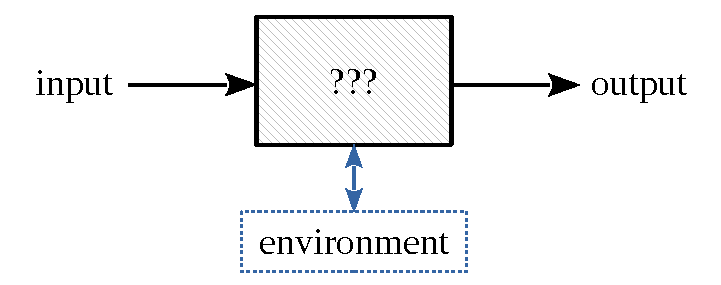
\includegraphics[width=0.9\linewidth]{images/blackbox} 
%    \caption{Black-box approach}
%    %\label{fig:sub1}
%  \end{subfigure}%
%  \begin{subfigure}{.5\textwidth}
%    \centering
%    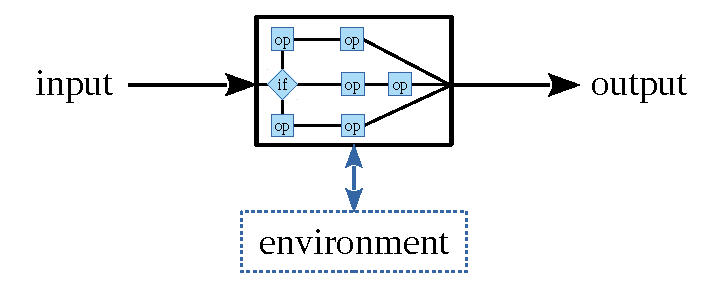
\includegraphics[width=0.9\linewidth]{images/whitebox} 
%    \caption{White-box approach}
%    %\label{fig:sub2}
%  \end{subfigure}
%  %\label{fig:example-symbolic-execution}
%  \vspace{-3mm}
%\end{figure}
%
%\paragraph{Taken from old Overview}
%
%Symbolic execution has been originally introduced in~\cite{K-CACM76} and~\cite{H-TSE77}. A good introduction to symbolic execution is presented in~\cite{KLEE-OSDI08}.\mynote{Extend this paragraph}
%%(while~\cite{EXE-CCS06} is a previous effort of the same authors).
%\cite{SAGE-NDSS08} is one successful story of symbolic execution. \cite{SAB-SP10} presents a neat formalization of symbolic execution and of taint analysis as well.
%

% !TEX root = main.tex

\section{Overview}

Symbolic execution has been originally introduced in~\cite{K-CACM76} and~\cite{H-TSE77}. A good introduction to symbolic execution is presented in~\cite{KLEE-OSDI08}.\mynote{Extend this paragraph}
%(while~\cite{EXE-CCS06} is a previous effort of the same authors).
\cite{SAGE-NDSS08} is one successful story of symbolic execution. \cite{SAB-SP10} presents a neat formalization of symbolic execution and of taint analysis as well.

\subsection{Motivation}

Symbolic execution is a static analysis technique that has been introduced to perform automatic testing of
%complex
software. For instance, let us consider the C function shown in Figure~\ref{fig:example-1}. A critical operation performed in this code is the division on line 10. In principle, testing techniques such as random testing can generate bottomless input tests for this function, although it is unlikely that the inputs which make this code crash are effectively picked up by these techniques\mynote{Fuzzing?}. Indeed, albeit this code is relatively simple, too many assignments to the input values {\tt a}, {\tt b}, and {\tt c} are possible. Each {\tt int} input variable can be assigned to $2^{32}$ distinct values, but only those leading to $x + y + z - 3 = 0$ would make the code crash.

Symbolic execution overcomes common limitations of random testing techniques by evaluating a piece of code using {\em symbols} instead of concrete values for the inputs. The intuition behind it is to consider classes of input values instead of single instance values. Before analyzing how symbolic execution can identify the proper inputs which will make the function {\tt foobar} crash, we now introduce a few basic definitions.

\subsection{A Simple Execution Model}
\label{simple-execution-model}

Symbolic execution is a methodology for executing a program symbolically. In particular, every local or global variable is associated with a {\em symbol} of the form $\alpha_i$.  At any point of the execution, a symbolic engine has to maintain an execution state.

%\paragraph{Symbol} Any local or global variable is associated to a symbol $\alpha_i$. 
\paragraph{Execution state} An execution state $(stmt,~pc)$ is composed of two elements:
\begin{itemize}
  \item $stmt$: the statement to evaluate
  \item $pc$: a collection of path constraints, i.e., a set of assumptions made over the symbols $\alpha_i$ in order to reach $stmt$. Initially $pc$ is empty, and is thus trivially satisfied.
\end{itemize}

As in general every memory location can be associated with a symbol, an execution engine typically maintains also a {\em memory mapping} $M$ for storing constraints over different symbols.\mynote{Rephrase}

\paragraph{Execution model} In this section we discuss a simple language supporting assignments, conditional branches and jumps. A discussion of more complex constructs such as $call$, $return$, $while$, or $for$ will be provided in Section~\ref{example-discussion}. Depending on the kind of the statement $stmt$, the execution engine modifies the state as follows:
\begin{itemize}
  \item (constant assignment) $\alpha_i = c$: when a constant value $c$ is assigned to a variable associated to the symbol $\alpha_i$, $pc$ is extended by adding a constraint on $\alpha_i$:\mynote{Redundant?}
    \[ pc \gets pc \wedge \alpha_i = c\]
  \item (assignment) $\alpha_i = e$: when an expression $e$ is assigned to a symbol $\alpha_i$, $pc$ is extended by adding a constraint on $\alpha_i$:
    \[ pc \gets pc \wedge \alpha_i = e\]
  where $e$ can be any expression, involving unary or binary operators, over symbols and constants.
  \item (conditional branch) {\tt if} $e$ {\tt then} $s_{true}$ {\tt else} $s_{false}$: $pc$ is evaluated. Two scenarios are possible:
    \begin{itemize}
      \item (non-forking) $e$ is evaluated as always true or false under the assumptions in $pc$: the proper branch is taken, and symbolic execution advances to $s_{true}$ or $s_{false}$ accordingly;
      \item (forking) $e$ cannot be evaluated without instantiating values for one or more symbols in it: the symbolic execution process is forked, creating two execution states:
        \[ (s_{true}, pc_{true}) \text{ where } pc_{true} = pc \wedge e \]
        \[ (s_{false}, pc_{false}) \text{ where } pc_{false} = pc \wedge \neg e \]
    \end{itemize}
    Symbolic execution proceeds on both states in parallel.
  \item (jump) {\tt goto} $s$: execution state is updated to advance symbolic execution to $s$. 
  %\item (other constructs) A discussion of other constructs such as $call$, $return$, $while$, or $for$ is provided in Section~\ref{example-discussion}. 
\end{itemize}

\subsection{Example}
\label{symbolic-execution-example}

\begin{figure}[t]
\begin{lstlisting}[basicstyle=\ttfamily\small]
              1.  int foobar(int a, int b, int c) {
              2.    int x = 0, y = 0, z = 0;
              3.    if (a != 0)
              4.      x = -2;
              5.    if (b < 5) {
              6.      z = 2;
              7.      if (a == 0 && c != 0)
              8.        y = 1;
              9.    }
             10.    return a / (x + y + z - 3);
             11.  }
\end{lstlisting}
\label{fig:example-1}
\caption{Example: a very simple C function}
\end{figure}

\begin{figure}[t]
  \centering
  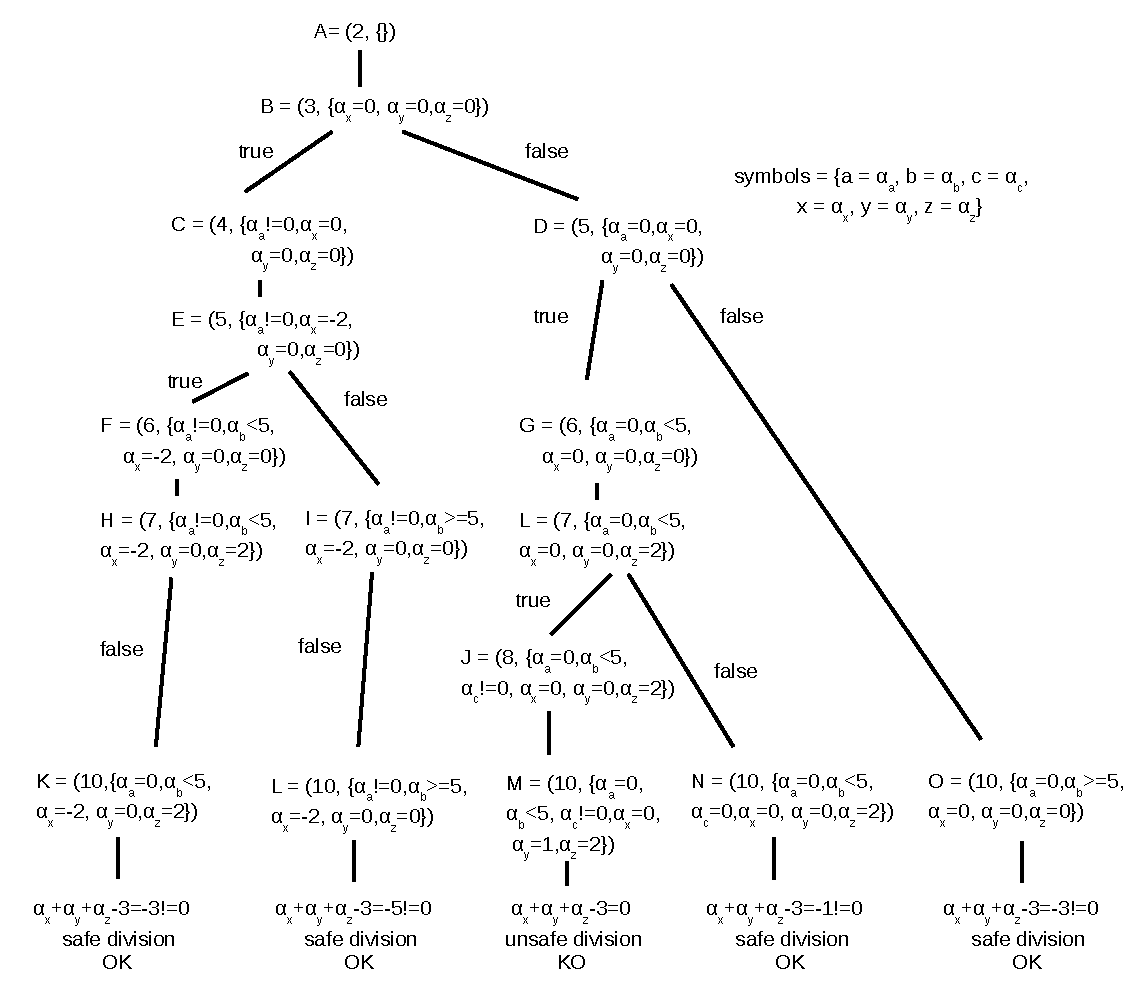
\includegraphics[width=1.0\columnwidth]{images/example} 
  \caption{Symbolic execution tree of the function {\tt foobar}. Each execution state is labeled with an alphabet letter. Side effects on execution states are highlighted in gray. Leaves are evaluated against division by zero error. For the sake of presentation the conjunction of constraints is shown as a list of constraints. }
  \label{fig:example-symbolic-execution}
\end{figure}

A symbolic execution of the function {\tt foobar} is shown in Figure~\ref{fig:example-symbolic-execution}. Initially, a new symbol is introduced for each input argument and for each local variable. For the sake of the presentation, we associate a symbol $\alpha_{var}$ with each variable $var$. 
Moreover, we assume that the set of local\mynote{locals only right? I added "at each point"} variables in use at each point by the function is known. In general, obtaining this information may be non trivial, and symbols are typically introduced when statements defining the variables are reached.
%Moreover, we have assumed to know the set of local variables used by the function. In general, obtaining this information may be non trivial and thus it it common to introduce symbols related to local variables only when the statements defining the variables are evaluated.
We also maintain a mapping table to track the mapping between variables and symbols. 

The first statement of the function is located at line 2. For this reason, the initial execution state $A$ is given by $(2, \{\})$ where the path constraint set is empty as no assumption is made on any symbol. After executing line 2,  $pc$ is updated by adding constraints on the value of $\alpha_x$, $\alpha_y$, and $\alpha_z$ (execution state $B$). Line 3 contains a conditional branch: since the condition cannot be uniquely determined based on the current set of assumptions, the execution is forked. Depending on the branch taken, a different statement is evaluated next and different assumptions are made on the symbol (execution states $C$ and $D$). On the other hand, when a condition can be uniquely determined (e.g., as in execution state $H$), it is sufficient to follow only the relevant branch (e.g., going to state $L$ from $H$), thus pruning unrealistic execution states. 

After expanding every execution state until the statement on line 10 is reached, we can check which input values for parameters {\tt a}, {\tt b}, and {\tt c} can make the function {\tt foobar} crash as a consequence of a division-by-zero operation. Analyzing execution states $\{L, M, N, O, P\}$, we can conclude that only $N$ can lead to an unsafe operation. The path constraint set for $N$ thus defines\mynote{implicitly defines?} the set of inputs that are unsafe for {\tt foobar}. Indeed, any input values for $\alpha_a$, $\alpha_b$, and $\alpha_c$ such that:
 \[ \alpha_a = 0 \wedge \alpha_b < 5 \wedge \alpha_c \neq 0 \]
will make the function crash. An instance of unsafe input parameters for {\tt foobar} can determined exploiting a constraint solver (i.e., an oracle able to resolve constraints). For instance, given the execution state $N$, a solver may come up with the values $a = 0$, $b = 1$, and $c = 0$. Notice\mynote{Say earlier?} that a constraint solver is also needed when evaluating the satisfiability of branch conditions.

\subsection{Discussion}
\label{example-discussion}

The example described in Section~\ref{symbolic-execution-example} shows the effectiveness of symbolic execution in identifying {\em all} the possible unsafe input values that can trigger a crash due to an unsafe division performed at line 10. This is achieved through an exhaustive exploration of all the possible execution states. For this reason, symbolic execution is a sound and complete methodology from a theoretical perspective. Soundness guarantees that input values deemed as unsafe are actually unsafe, and completeness implies that all possible unsafe inputs will be found. However, challenges that symbolic execution has to face when processing real-world code can be significantly more complex compared to those from our toy example of Figure~\ref{fig:example-1}. Several observations and questions naturally arise:

\begin{enumerate}

  \item (objects) {\em How does symbolic execution handle arrays or other more complex objects?} \\
  In general, any arbitrary complex object can be seen as an array of bytes, where each byte is associated with a distinct symbol. In principle, even a C {\tt int} variable can be seen as an array of four bytes.\mynote{Cosa intendiamo qui?} However, it is convenient to exploit structural properties of the data when possible (e.g., by statically analyzing the source code). For instance, for object-oriented languages the search performed by symbolic execution can be refined taking advantage of relational bounds on class fields.

  \item (loops) {\em How does symbolic execution handle loops?} \\
  In the execution model presented in Section~\ref{simple-execution-model} a loop can be encoded as a combination of conditional branches and $goto$ statements. This transformation is frequent when lowering a high-level language like C to an intermediate representation or native code. When the number of loop iterations cannot be determined in advance (e.g., it depends on an input parameter), for a symbolic execution engine choosing how many iterations should be analyzed becomes critical. The naive approach of unrolling iterations for every valid index bound leads to a very large number of states. It is possible to limit the number of iterations to $k$, thus trading speed for completeness, or when loop invariants can be inferred through static analysis they can be used to merge equivalent states (\mynote{Recuperare citazione}e.g., when differences are not observable outside the loop body).

  \item (subroutines) {\em How does symbolic execution handle subroutines?} \\
  Our execution model does not handle invocation of subroutines (i.e., a $call$ statement). \mynote{Extend this paragraph} A way to extend it to support subroutines is to provide the execution state with a simple execution stack.

  \item (recursion) {\em How does symbolic execution handle recursion?} \\
  Consider, as an example, the code:
    \begin{lstlisting}[basicstyle=\ttfamily\small]
    1.  int bar(int n) {
    2.    if (n >= 0) 
    3.      return 0;
    4.    return 1 + sum(n - 1);
    5.  }
    \end{lstlisting}
  Assuming that an execution stack has been added to the state, we observe that this code can easily lead to a very large number of execution states (i.e., a new state is subsequently created every time the branch on line 2 is not taken). As an {\tt int} variable can have up to  $2^{31} - 1$ positive values, symbolic execution has to create as many execution states to cover all the possible execution paths.
 %Indeed, the number of executions states is related to the number of times that the conditional branch on line 2 is not taken. 
 
  \item (environment) {\em How does symbolic execution handle interaction with the environment}? \\
  Real-world applications interacts constantly with the environment (e.g., filesystem, network) through libraries or system calls. A crucial aspect of these interactions is that they may cause side-effects
% on the environments 
(e.g., creation of a file)
%or initialization of a memory area
that must be taken into account, as they may later affect the 
%actual
execution of the code. Evaluating any possible outcome of an interaction is typically not feasible due to the large number of possibly generated execution states, only a small number of which can actually happen in a non-symbolic scenario. Hence, it is common to create models for popular library and system routines that help the symbolic execution engine to consider only significant outcomes.

  \item (state space explosion, path selection) {\em How does symbolic execution deal with path explosion}? \\
  A relatively simple code such as function {\tt foobar}, which is composed by less 12 lines of code, has generated 16 execution states, where $5$ out of $16$ are independent\mynote{Independent?} and must be checked to determine possible unsafe input values. Although this could seem a reasonable number of states, language constructs such as loops may contribute to increase the number of states exponentially. For this reason, it is unlikely that a symbolic execution engine is able to exhaustively explore all the possible execution states within a reasonable amount of time. In practice, heuristics are used to guide exploration and prioritize certain states first (e.g., to maximize code coverage), hoping this would lead to interesting discoveries. Also, a symbolic execution engine should implement efficient mechanism for evaluating multiple execution states in parallel without running out of resources.
  %In practice, several heuristics must be exploited to prioritize evaluation of some states, hoping to still be able to spot interesting things. Moreover, the symbolic execution engine should include efficient mechanism for efficiently evaluating in parallel different execution states without running out of computational resources.

  \item (constraint solver) {\em What can a constraint solver do in practice?}
  %{\em What is a constraint solver in practice}? \\
 Constraint solvers suffer from a number of limitations. Typically, they can handle complex constraints in a reasonable amount of time only if they are made of linear expressions over their constituents. Symbolic execution engines typically implement a number of optimizations to make queries as much {\em solver-friendly} as possible, for instance by splitting queries in independent components to process separately or by performing algebraic simplifications.

  \item (binary code) {\em What are the disadvantages of symbolically executing binary code}? \\
  The example presented in Section~\ref{symbolic-execution-example} is written in C. This does not imply that symbolic execution cannot be performed directly on binary code, which in several scenarios is the only available representation of a program. However, having the source code of an application makes symbolic execution significantly easier, as it can exploit high-level properties (e.g., object shapes) that can be inferred by statically analyzing the source code.
  %(e.g., the maximum size of a buffer or the number of iterations for a loop).
   
\end{enumerate}
%Depending on the specific application context of symbolic execution
Depending on the specific context in which symbolic execution is used, different choices and assumptions are made to address the questions highlighted above. Although they typically affect soundness or completeness, in several scenarios a partial exploration of the space of possible execution states is typically sufficient to reach the goal\mynote{Better example?} (e.g., identify a crashing input for an application) with a limited time budget.

%different choices and assumptions are made to address the above questions. Although soundness and completeness of symbolic execution may be negatively affected by these choices, there are several application scenarios where a partial exploration of the possible execution states is sufficient for reaching the ultimate goal (e.g., identify a single input that crashes an application).


%%%%%%%%%%%%%%%%%%%%%%%%%%%%%%%%%%%%%%%%%%%%%%%%%%%%%
\section{Memory model}
\label{memory-model}

A crucial aspect of symbolic execution is how the memory should be modeled. In other words, a symbolic engine may see symbols as distinct objects (i.e., each symbol is a distinct array of a specific size) or as pointers to a flat memory (i.e., index-based memory). Although the latter approach may seem more natural since it is akin to a concrete execution model, the former has been proved to be very effective in many scenarios since the symbolic constraints generated when using this approach are {\em easier} to parse for some solvers.

\subsection{Index-based memory}
\begin{itemize}
  \item memory is a map $\pi : I \to E$ from 32-bit indices ($i \in I$) to expressions ($e \in E$)
  \item load expressions $e = load(\pi, i)$: $i$ indixes $\pi$ and the loaded value $e$ represents the contents of the $i$-th memory cell
  \item store expressions $store(\pi, i, e)$: a new memory $\pi'$ where $i$ is mapped to $e$, i.e., $\pi' = \pi[i \gets e]$
\end{itemize}
When using this memory model, handling of arbitrary symbolic indices is notoriously hard, since a symbolic index may reference any cell in memory. Two approaches can be pursued: (a) concretization of the index where only a single value is evaluated for the index (see Section~\ref{concolic-execution} for more details), (b) fully symbolic memory where any possible value for the index is evaluated (e.g., \cite{BAP-CAV11}). The former is often excessively limiting (many paths are pruned away), while the latter is hard to make scalable. To overcome the limitations of both approaches, \cite{MAYHEM-SP12} models memory {\em partially}: symbolic writes are always concretized, while symbolic reads are allowed to be modeled symbolically.

\paragraph{Memory objects} Whenever there is a symbolic read, an immutable memory object $\mathcal{M}$ is generated:  it contains all values that could be accessed by the index, i.e., $\mathcal{M}$ is a partial snapshot of the global memory $\pi$. In practice, \cite{MAYHEM-SP12} reasons on $\mathcal{M}[i]$ instead of reasoning on $\pi[i]$, since the former is typically smaller than the latter.

\paragraph{Memory object bounds resolution}\mynote{Move paragraphs to Section~\ref{constraint-optimizations}?} \cite{MAYHEM-SP12} trades accuracy with scalability by resolving the bounds $[\mathcal{L}, \mathcal{U}]$ of the memory region, where $\mathcal{L}$ is lower and $\mathcal{U}$ is the upper bound for the index $i$. Initially, $\mathcal{L} \in [0, 2^{32}-1]$. The solver is used to test if $i < \frac{2^{32}-1}{2}$ makes the path constrains unsatisfiable. If satisfiable then $\mathcal{L} \in [0, \frac{2^{32}-1}{2}]$, otherwise $\mathcal{L} \in [\frac{2^{32}-1}{2}, 2^{32}-1]$. The same strategy is repeated as much as possible. This is akin to a binary search algorithm. Whenever the bounds become reasonable, a memory object is generated. Unfortunately, there several cases where the bounds cannot be narrowed down drastically and thus other techniques can be used:
\begin{itemize}
  \item {\em value set analysis (VSA)}
  \item {\em refinement cache}
  \item {\em lemma cache}
  \item {\em index search trees (IST)}
  \item {\em bucketization with linear functions}
\end{itemize}
Whenever the size of the memory object exceeds a threshold (e.g., $|\mathcal{M}| \geq 1024$), then~\cite{MAYHEM-SP12} concretizes the index. However, instead of choosing a random value for the index, it tries to assign some {\em interesting} value (e.g., test it if it makes sense for it to be equal to an invalid memory address which can be exploited for security purposes).

\subsection{Object-based memory}

\cite{STP-TR07} is a decision procedure for bitvectors and arrays. Memory is seen as untyped bytes. Three data types are available:
\begin{itemize}
  \item {\em booleans}
  \item {\em bitvectors}: a fixed-length sequence of bits
  \item {\em arrays of bitvectors}
\end{itemize}
Most linear and non-linear operations are mapped to bitvector constraints. Conditional branches are transformaed into {\em multiplexers}, which are similar to C ternary operator. Bitvector operations are translated into operations to individual bits. Floating-points data types are not supported. Expresions types:
\begin{itemize}
  \item {\em formulas}, which have boolean values. They are converted into DAGs of single bit operations, where expressions with identical structure are represented uniquely (an hash table is maintain to track of existing expressions and lookups are performed on it when a new expression is created).
  \item {\em terms}, which have bitvectors values. They are converted into vectors of boolean formulas consisting entirely of single bit operations.
\end{itemize}

\paragraph{Mapping C code to STP primitives} Each C data block is represented symbolically as an array of 8-bit bitvectors. Typed operations in C generated constraints on the symbolic data (i.e., typeness is not actually known to~\cite{STP-TR07}). A mapping table is maintained to track symbolic data:
\begin{itemize}
  \item each input array $b$ is associated to a symbolic identically-size array $b_{sym}$ (i.e., the address of the C variable $b$ is mapped to the symbolic array $b_{sym}$ that is composed by $|b|$ 8-bit elements)
  \item $v = e$: an assignment expression, where $e$ is an expression that involves one or more symbolic data, adds a mapping between the address of $v$ and the generated symbolic expression $e_{sym}$. If $v$ is overwritten with a constant value or deallocated then this mapping is removed.
  \item $b[e]$: $b_{sym}$ is allocated, initializing it with the (constant) contents of $b$ (only if $b$ is actually initialized by a previous C statement). A mapping is added until $b$ is not deallocated.
\end{itemize}

\paragraph{Expression evaluation} An expression $e$ that contains some symbolic data can be seen as:
\[ l_1~~op_1~~l_2~~op_2~~l_3~~... \]
Each $l_i$ is evaluated in the following way:
\begin{itemize}
  \item if $l_i$ is concrete: the concrete value is used in the expression (e.g., if 4-byte $b$ is equal to 4 then the constant $000000...0100$ is used)
  \item otherwise: a concatenation of all the symbolic bytes of $l_i$ is used (e.g., $b_{sym}[0] @b_{sym}[1] @ $ $b_{sym}[2] @ b_{sym}[3] @ ...$)
\end{itemize}
Pointers are seen as array reference at some offset. This means that allocation sites as well as pointer arithmetic expressions must be instrumented in order to track where a pointer can point to. Notice that double dereferences ({\tt **p}) force~\cite{STP-TR07} to concretize the first dereference ({\tt *p}). 

\paragraph{Fast array transformations}\mynote{Move paragraphs to Section~\ref{constraint-optimizations}?} Some transformations are needed to make\cite{STP-TR07} reason only on a purely functional language. In particular:
\begin{itemize}
  \item {\em read-over-write}: eliminates all write operations
    \[ read(write(A, i, v), j) \implies ite(i = j, v, read(A, j)) \]
    where $ite(a,b,c)$ is a ternary operator (i.e., if $a$ then $b$ else $c$). Notice that a write of a location without a subsequent read of the same location can be ignored.
  \item {\em read elimination}:
    \[ (read(A, i) = e_1) \wedge (read(A, j) = e_2) \]
    will be transformed in:
    \[ (v_1 = e_1) \wedge (v_2 = e_2) \wedge (i=j \implies v_1 = v_2) \]
  \item {\em array substitution optimization}
  \item {\em array-based refinement}
  \item {\em simplifications}: boolean or mathematical identities
\end{itemize} 

\paragraph{Optimizations}\mynote{Move paragraphs to Section~\ref{constraint-optimizations}?} Other optimizations are applied:
\begin{itemize}
  \item {\em constraint caching}: cache solver results and reuse them
  \item {\em constraint independence}: tracks constraints into multiple independent subsets of constraints, This helps the system discards irrelevant constraints and adds additional cache hits.  
\end{itemize}

\section{Loops}

Loops can easily lead to the path explosion problem: any iteration of a loop can be seen as a {\tt IF-GOTO} statement. Example taken from~\cite{CS-CACM13}:
    \begin{lstlisting}[basicstyle=\ttfamily\small]
    1.  int N = sym_input(); // e.g., read
    2.  while (N > 0) {
    3.    N = sym_input();  
    4.  }
    \end{lstlisting}
The path constraint set of any final state will contain:
  \[ \left ( \bigwedge_{i \in [1, n]]} N_i > 0 \right ) \wedge (N_{n+1} \leq 0) \]
where $N_i$ is the symbol introduced at the i-th iteration.\\

For this reason, it is common to specifically deal with them:
\begin{itemize}

  \item {\em preconditions}: a technique to make it easier to perform symbolic execution on loops is through imposing some preconditions, e.g., use static analysis techniques to understand number of iterations for a loop. See Section~\ref{precontioned-symbolic-execution} for more details.

  \item {\em fixed exploration}: depending on the goal, a symbolic engine may decide to fully explore a loop (e.g., see heuristics presented in~\cite{AEG-NDSS11} and discussed in Section~\ref{heuristics}) or explore only a fixed number of iterations (e.g., up to 3 iterations) in order to avoid path explosion.

  \item {\em approximations}: effects of a loop are often approximated using {\em fixpoints} (e.g., in~\cite{KKM-USEC05,BNS-SP06,CFB-ACSAC06}). A fixpoint F is an approximation of the effect of loop body on an execution state. F approximates the state after the execution of loop whenever the initial state before the loop was F (?). Transforming an execution state to a fixpoint state is defined as widening. Construction of the fixpoint:
  \begin{itemize}
    \item S1: state after first iteration
    \item S2: state after second iteration
    \item compare S1 and S2: assign bottom to each symbol that has been altered
    \item repeat until there is no difference between Si and Si+1
    \item if there is a branch inside the loop, then either the branch is known or its condition is on a symbol which has been assign to bottom. In this case, two parallel states are created and then compared.
  \end{itemize}

\end{itemize}

Notice that detection/analysis of loops can be done using techniques such as~\cite{SGL-TOPLAS96} (e.g., in~\cite{CFB-ACSAC06}).

\section{Subroutines and recursion}

\section{Interaction with environment}

Environment can be seen as an input source. Since it can be unfeasible to analyze all possible interactions with the environment, it is common to model these interactions, emulating their behaviors and their side-effects. The main intuition is that models understand the semantics of the desired actions well enough to generate the required constraints.\\

\cite{KLEE-OSDI08}:
\begin{itemize}
  \item {\em file system}: operations on concrete files are actually performed. Operations on symbolic files are emulated modeling a simple symbolic file system, which is private for each execution state. Symbolic file system is a directory with $N$ symbolic files. Users specify both the number of files and their sizes. Any operation on a unconstrained symbolic file will generate $N+1$ branches: one for each symbolic file, plus one for a failing scenario. Emulation done at library level, not system call level. This make symbolic execution simpler (no need to symbolically execute library code) but assumption that library code is correct. If needed, library code is tested separately.
  \item {\em environment failures}: \cite{KLEE-OSDI08} emulates failures (e.g., failures of {\tt write}). This is optional since some applications may be not sensitive to environment failure.
  \item {\em re-running test cases}: inputs which may crash an application may depend on the environment failures. To force concrete execution towards failures, \cite{KLEE-OSDI08} exploits {\tt ptrace}.
\end{itemize}

\cite{AEG-NDSS11}:
\begin{itemize}
  \item {\em symbolic files}: emulation of {\tt open}, {\tt read}, {\tt write}, and similar other system calls. Similar to~\cite{KLEE-OSDI08}.
  \item {\em symbolic sockets}: emulation of {\tt socket}, {\tt bind}, {\tt accept}, {\tt send}, and similar other system calls. 
  \item {\em environment variables}: a complete summary of all possible results (concrete values, fully symbolic, and failures) of {\tt get\_env}.
  \item {\em library function calls and system calls}: emulation of more than 70 library routines and system calls. In particular, formatting functions (e.g., {\tt fprintf}) are emulated to capture buffer overflows.
\end{itemize}

\cite{DART-PLDI05}: external interfaces are extracted by analyzing library and system calls, then random results are returned (compliant with the type).

\section{State space explosion}

The main challenge with symbolic execution is managing the state space explosion problem. Since symbolic execution forks off a new interpreter at every (undecidable) branch, the total number of interpreters is exponentially in the number of of branches.

\subsection{Preconditioned symbolic execution}
\label{precontioned-symbolic-execution}

\cite{AEG-NDSS11} has proposed {\em preconditional symbolic execution} as a novel method to target symbolic execution towards certain subset of the input state space. The state space subset is determined by the precondition predicate $\Pi_{prec}$: inputs that do not satisfy $\Pi_{prec}$ will not be explored. The intuition for preconditioned symbolic execution is that we can narrow down the state space we are exploring by specifying exploitability conditions as a precondition, e.g., all symbolic inputs should have the maximum size to trigger buffer overflow bugs. The main benefit from preconditioned symbolic execution is simple: by limiting the size of the input state space before symbolic execution begins, we can prune program paths and therefore explore the target program more efficiently.
Note that preconditions cannot be selected at random. If a precondition is too specific, we will detect no bugs or exploits; if it is too general, we will have to explore almost the entire state space. %Thus, preconditions have to describe common characteristics among exploits (to capture as many as possible) and at the same time it should eliminate a significant portion of non-exploitable inputs.\\

Preconditioned symbolic execution enforces the precondition by adding the precondition constraints to the path predicate during initialization. Adding constraints may seem strange since there are more checks to perform at branch points during symbolic execution. However, the shrinking of the state space -- imposed by the precondition constraints -- outweighs the decision procedure overhead at branching points. When the precondition for a branch is unsatisfiable, we do no further checks and do not fork off an interpreter at all for the branch.% We note that while we focus only on exploitable paths, the overall technique is more generally applicable.\\

\paragraph{Preconditions} Kinds of preconditions:
\begin{itemize}
  \item {\em None}. There is no precondition and the state space is explored as normal.
  \item {\em Known Length}. The precondition is that inputs are of known maximum length. Static analysis techniques can be used to automatically determine this precondition.
  \item {\em Known Prefix}. The precondition is that the symbolic inputs have a known prefix.
  \item {\em Concolic Execution}. Concolic execution [24] can be viewed as a specific form of preconditioned symbolic execution where the precondition is specified by a single program path as realized by an example input. For example, we may already have an input that crashes the program, and we use it as a precondition to determine if the executed path is exploitable. See Section~\ref{concolic-execution} for a more detailed discussion of this technique.
\end{itemize}

\paragraph{An example} Consider the example:

\begin{lstlisting}[basicstyle=\ttfamily\small]
    // N symbolic branches 
    if (input[0] < 42) [...]
    [...]
    if (input[N - 1] < 42) [...]

    // symbolic loop
    strcpy(dest, input); 

    // M symbolic branches
    if (input[N + 1] < 42) [...]
    [...]
    if (input[N + M - 1] < 42) [...]
    \end{lstlisting}
where {\tt input} is an array of {\tt S} bytes. Impact of preconditions:
\begin{itemize}
  \item {\em None}. No constraint is added. State space is $2^N \cdot S \cdot 2^M$.
  \item {\em Known Length}. For instance, we add constraint that $(S - 1)$ bytes of {\tt input} are not equal to \textbackslash0. Since the symbolic loop is known, then the state space is reduce to $2^N \cdot 2^M$.
  \item {\em Known Prefix}. For instance, we add constraint that the $P$ bytes of {\tt input} are known ($P < N < S$). E.g., fixed header string). Since first $P$ branches and first $P$ iterations are concrete, then state space is $S \cdot 2^{N-P} \cdot 2^M$.
  \item {\em Concolic Execution}. We decide the exact values for all bytes of {\tt input}. Input space is $1$.
\end{itemize}

\subsection{Dynamic symbolic execution}


\paragraph{Concolic execution}
\label{concolic-execution}
{\em Concolic execution} has been originally introduced in~\cite{DART-PLDI05} and then refined by~\cite{CUTE-FSE13}. A common disadvantage of symbolic execution is that the state space can be exponential. Moreover, even when the state space is tractable it may happen that complex constraints need to be solved but these constraints are too complex for the actual solver (e.g., non-linear constraints are typically hard to solve). For this reason, it is common to exploit concolic execution. Different scenarios:
\begin{itemize}
  \item {\em Use concolic execution to generate useful (random) inputs.} Starts concrete execution using a random (concrete) input and for each taken branch tracks the input constraints by observing the branch condition. When the execution is completed, restart another concrete execution using a different concrete random input that is compliant with the constraints but explore a new path. It is sufficient to negate a single constraint given by a conditional branch, to explore a different path. Keep track of taken branches with binary values. An algorithm for maximizing coverage is proposed in~\cite{DART-PLDI05}. Notice that the symbolic execution is performed in parallel with the concrete execution. Related examples are~\cite{SAGE-NDSS08,DRILLER-NDSS16}. In particular,~\cite{DRILLER-NDSS16} is an example of {\em symbolic-assisted fuzzing}: their technique temporarily exploits concolic execution only when a fuzzer cannot generate a valid input to explore an uncovered branch.

  \item {\em Use concolic execution to overcome unsolvable constraints}. Assume to start a concrete execution with a concrete input and in parallel symbolically execute the same program. Whenever a set of constraints cannot be solved by the constraint solver, then use the concrete value to proceed into at least one branch. Example taken from~\cite{CS-CACM13}:
    \begin{lstlisting}[basicstyle=\ttfamily\small]
    int non_linear(int v) {
      return (v * v) % 50;
    }
    \end{lstlisting}
  The non-linear operation inside this function can be hard for a solver. Using a concrete execution, the engine can overcome this problem, but then the precision and completeness may be affected.

  Notice that the use of concrete values can also avoid to perform alias analysis on pointers, which is typically very expensive. Whenever meaningful, \cite{DART-PLDI05} tries to test both valid (not {\tt NULL}) and invalid ({\tt NULL}) input pointers in order to maximize bug detection. However~\cite{DART-PLDI05} will never artificially negate a branch if that condition cannot be exercised using a concrete input. In other words, both branches of an {\tt if} statement are considered only if they are both meaningful (more precisely: \cite{DART-PLDI05} is able to generate a valid input). Notice that~\cite{DART-PLDI05} may generate an input using a solver by considering only a subset of branch constraints. For instance, consider constraints ($C_1, C_2, C_3$) given by three nested branches: if $C_1$ is non linear (hard to solve), it needs only to generate a random input for taking $C_1$ and then use the solver for exploring path given by $(C_2, C_3)$. A traditional symbolic execution engine may get stuck at $C_1$ and give up after some time on {\em all} the derived path. Notice that whenever a concrete input is used to overcome a hard constraint, the overall approach become incomplete.

\end{itemize} 

\paragraph{An example}\mynote{Improve this discussion} Given a concrete input, an application will execute only a subsets of its basic blocks $B_i$. Moreover, they will be executed following a specific order. For instance, the program execution shown in Figure~\ref{fig:example-concrete-execution}a has executed the sequence of basic blocks $\{B_1, B_2, B_4, B_6\}$. Other blocks, such as $B_3$, have not been executed due to non-taken branches. Driven by the concrete execution, a symbolic execution engine may trace symbolic constraints on the taken branches and then generate an input that forces the execution to take a never-taken branch. For instance, if the symbolic execution engine may want to generate an input that executes basic block $B_5$, then it traces the constraints on the two taken branches and then negate the constraint on the branch that leads the execution toward $B_5$. Figure~\ref{fig:example-concrete-execution}b provides the logical steps performed by the engine.

\begin{figure}[t]
  \vspace{-3mm}
  \centering
  \begin{subfigure}{.5\textwidth}
    \centering
    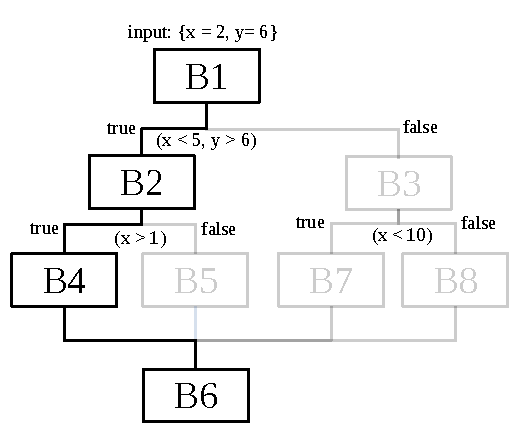
\includegraphics[width=0.9\columnwidth]{images/concrete-execution} 
    %\label{fig:sub1}
    \vspace{15mm}
    \caption{}
  \end{subfigure}%
  \begin{subfigure}{.5\textwidth}
    \centering
    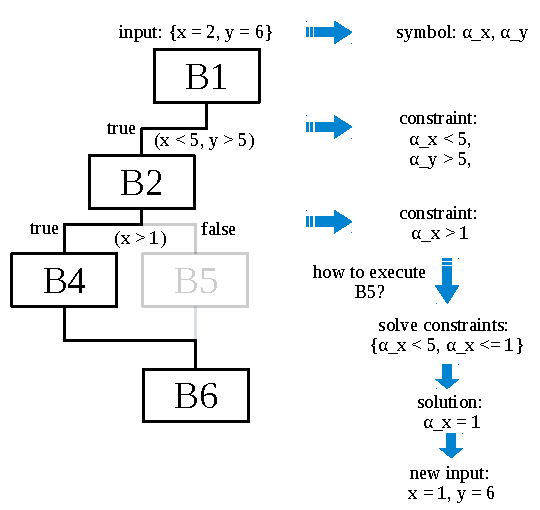
\includegraphics[width=1.0\columnwidth]{images/concolic-execution} 
    %\label{fig:sub2}
    \caption{}
  \end{subfigure}
  \caption{(a) a concrete execution of a program. Only a subset of basic blocks is executed. The sequence of executed basic blocks is $\{B_1, B_2, B_4, B_6\}$. (b) concolic execution for generating an input that executes $B_5$.}
  \label{fig:example-concrete-execution}
  \vspace{-3mm}
\end{figure}

%Errors related to concrete values and 
\paragraph{Execution-Generated Testing} {\em Execution-Generated Testing (EGT)} is the approach used by some papers (e.g.,~\cite{KLEE-OSDI08,EXE-CCS06}) that works by making a distinction between the concrete and symbolic state of a program: if an operation involves only concrete values, then the symbolic engine concretely execute it. This can allow symbolic execution to reason even over complex operation (e.g., non linear operations) if they involve only concrete values. EGT is often seen (\cite{CS-CACM13}) as a form of dynamic symbolic execution: this can be seen as more general term than concolic execution.

\subsection{Under-constrained symbolic execution} 

By isolating a function from the rest of the program, we can perform symbolic execution on it. The results from this analysis can be exploited when any other program is symbolically executed and a call to the function is present. However, detected errors in the isolated function may be false positives since some of the input values may never been valid when the function is actually executed in the context of the full program. {\em Under-constrained symbolic execution}~\cite{ED-ISSTA07} is a technique that performs symbolic execution of an isolated function but clearly marks which symbols are {\em under-constrained} to distinguish them from the {\em exactly-constrained} symbols.

Errors due to concrete values and exactly-constrained symbols are treated as true positives. Errors due to under-constrained are treated as true positives only if {\em all} solutions to the currently known constraints on the symbols cause the error to occur. Otherwise the negation of the error is added to the constraint set and the symbolic execution of the isolated function is continued. In other words, an error is reported if and only if it is {\em context-insensitive}. Notice that a symbol may initially be under-constrained and then become exactly constrained. For instance, consider the following piece of code:
    \begin{lstlisting}[basicstyle=\ttfamily\small]
    assert(a != 0); // no knowledge about this variable
    a = 0;          // from now on we know the value of a
    assert(a != 0); // we always hit this error: context-insensitive! 
    \end{lstlisting}
The first {\tt assert} will not trigger an error: indeed, there is at least one possible value for the symbol associated to {\tt a} that does not hit the error. Conversely, the second {\tt assert} will always trigger an error since {\tt a} has a concrete value and it's not under-constrained anymore.\\

Although this technique is not able to find {\em all} the possible errors in a function, it still can find interesting bugs. Moreover, since symbolically executing a full program may be unfeasible, this technique can make it feasible to test tons of line of code in a reasonable amount of time. In particular, this technique allows an engine to skip code: if a function or any other construct (e.g., a loop) may be troublesome for symbolic execution, it can be skipped by just marking the locations affected by it as under-constrained. However, a possible implementation issue is given by the propagation of under-constrained symbols: given the line of code {\tt if (s < t)}, if {\tt t} is under-constrained while {\tt s} is exactly constrained then when the symbolic execution is proceeded into the two possible branches, {\tt s} must be marked as under-constrained. Some optimization may be needed in order to minimize this propagation effect.

\paragraph{Under-constrained KLEE}\mynote{I will revise it (emilio)} In~\cite{UCKLEE-USEC15}, KLEE~\cite{KLEE-OSDI08} has been extended in order to support under-constrained symbolic execution . In particular, these are some of the main improvements:
\begin{itemize}
  \item {\em Lazy initialization.} Whenever there is a pointer that is not concrete and without any active constraint (i.e., it is unbound), it its value is checked against {\tt NULL} then two path are analyzed: (a) where the pointer is {\tt NULL} and (b) where the pointer is pointing to a freshly allocated block of memory, whose content is marked as unbound.This means that pointer aliasing is assumed to not occur. In both paths, the pointer is not longer unbound.  In path (b), any test against the pointer is known and dereferences will be successfully resolved. Lazy initialization is common for data structure and thus it is common to bound its maximum length (i.e., {\em k-bounding}) in order to prevent the engine from allocating an unbounded number of objects.
  \item {\em Patch checking.} The main goal of~\cite{UCKLEE-USEC15} is to detect if a patch has introduced new bugs. In order to do so, it symbolically executes two compiled versions of a function: $P$, the unpatched version, and $P'$, the patched version. If it finds any execution paths along which $P'$ crashes but $P$ does not (when given the same symbolic inputs), it reports a potential bug. Indeed, due to missing input preconditions, not all crashes are real bugs: if both $P$ and $P'$ crash on an input, then maybe the crash is given by the unknown preconditions. 
  \item {\em Pruning techniques.} Using a static cross-checker (that navigates the control-flow graph and marks differing basic block between $P$ and $P'$), \cite{UCKLEE-USEC15} prunes paths that have never executed a differing basic block and that cannot reach a differing basic block from their current program counter and call stack. Moreover, $P'$ is executed before executing $P$, allowing the system to prune paths that return from $P'$ without triggering an error, or that trigger an error without reaching different blocks.
  \item {Dealing with false positives.} Two approaches are pursued to limit false positives:
    \begin{itemize}
      \item {\em manual annotations}: examples are data types invariants or preconditions upon function calls.
      \item {\em automated heuristics}: {\em must-fail} heuristics identify errors that must occur for all input values following that execution path. For instance, {\em belief-fail} heuristic checks if a function contradicts itself (e.g., a code checks that a pointer is {\tt NULL} and then dereferences it). Another variation of must-fail heuristic is {\em concrete-fail} that an assertion failure or memory errors was triggered by a concrete condition or pointer.
    \end{itemize}
  \item {\em Rule-based checkers.} Several rule-based checkers have been built on top of UCKLEE. They do a similar job such as other dynamic tools (e.g., {\em memcheck} for memory leaks and uninitialized data) but reasoning on all possible paths, not just the concrete ones. Moreover, user inputs can be considered as fully constrained (i.e., no assumption is valid on it since the code should sanitize it). 
  \item {\em Optimizations.} Some optimizations:
    \begin{itemize}
      \item Symbolic objects have a symbolic size: whenever there is an access to the object content, the system verifies if the offset could exceed the object's symbolic size. whenever path is considered where the offset does not exceed the symbolic size, then a lower bound on the symbolic size is set.
      \item Some library functions (e.g., {\tt strlen}) have been replaced with variants that do not lead to path explosion
      \item Scores of rules to simplify symbolic expressions
      \item {\em lazy constraints}: defer evaluation of constraints using a solver as much as possible. For instance, if there is an hard constraint on branch, take both branches and if an error is found check if that branch was actually valid.
      \item function pointers should be made concrete by the user.
    \end{itemize}

\end{itemize}


\subsection{State merging}

Several static program analysis techniques such as abstract interpretation merge states corresponding to different paths into a state that over-approximates them. In a precise symbolic execution, however, merging is not allowed to introduce any approximation or abstraction, and therefore can only change formulas to have them characterize sets of execution paths. In other words, a merged state will be described by a formula that represents the disjunction of the formulas that would described the individual states if they were kept separate.

\paragraph{An example} Let's consider the following piece of code (taken from~\cite{VERITESTING-ICSE14}):\mynote{customize example and improve discussion}
    \begin{lstlisting}[basicstyle=\ttfamily\small]
    B1: if (x > 1) 
    B2:   y = 42;
    B3: else if (x < 42) 
    B4:    y = 17;
    B5: else ;
    B6: ;
    \end{lstlisting}
Then a symbolic execution engine may perform state merging in the following way:
\begin{figure}[H]
  \centering
  \vspace{-3mm}
  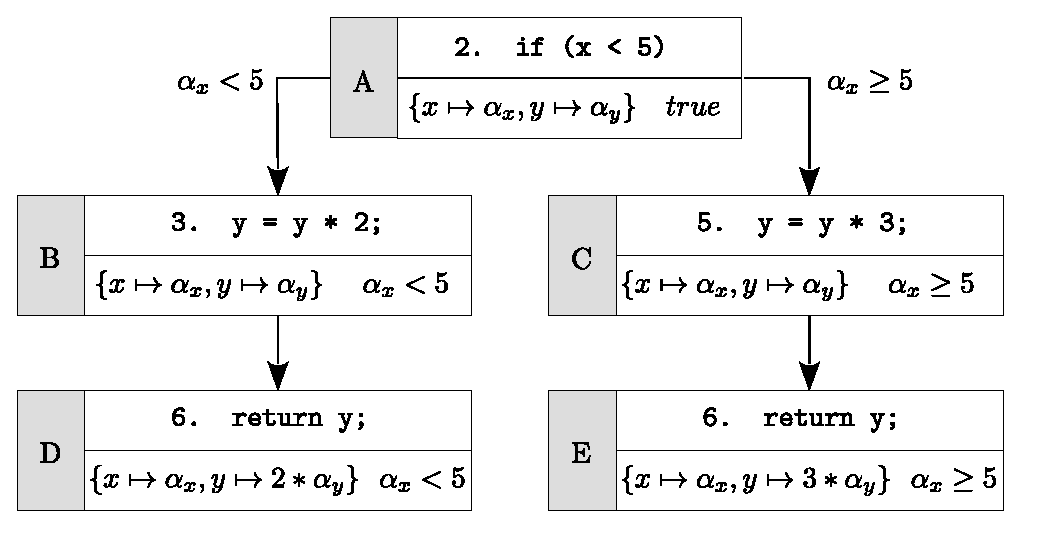
\includegraphics[width=0.65\columnwidth]{images/state-merging} 
  \vspace{-3mm}
  %\label{fig:example-symbolic-execution}
\end{figure}
where {\em ite} statements represents {\tt if-then-else} statements and $\bot$ stands for a non-taken branch.

\paragraph{Trade-off} Early work~\cite{G-POPL07,HSS-RV09} has shown that merging techniques effectively decrease the number of paths to explore, but also put a burden on constraints solvers, which typically encounter difficulties when dealing with disjunction. Merging can also introduce new symbolic expressions in the code, for instance when merging different concrete values from a conditional assignment into a symbolic expression over the condition. \cite{KKB-PLDI12} provides an excellent discussion of the design space of state merging techniques. At one end of the spectrum, search-based symbolic execution (as implemented, e.g., in~\cite{KLEE-OSDI08}) does not perform any merge. The other extreme is complete static state merging, implemented by verification condition generators, e.g, ~\cite{SATURN-POPL05,CALYSTO-ICSE08}), that combines states at join points after all the subpaths have been encoded.

\mynote{Function summaries}

\paragraph{Selective state merging} Intermediate merging solutions can adopt heuristics for driving both merging decisions and CFG exploration. Generating larger symbolic expressions and possibly extra solvers invocations can outweigh the benefit of having fewer states, leading to poorer overall performance~\cite{HSS-RV09,KKB-PLDI12}. Moreover, in order to maximize the opportunities for merging a symbolic execution engine should traverse the CFG in a topological order, which denies search exploration strategies aiming at prioritizing more ``interesting'' states over others.

Recent works (e.g., \cite{KKB-PLDI12} and \cite{VERITESTING-ICSE14}) have introduced novel techniques to tackle these issues: 
\begin{itemize}

  \item {\em query count estimation} identifies state merges that can reduce exploration time. This technique relies on a simple form of static analysis to identify how often each variable is used in branch conditions past any given point in the CFG. The estimate is used as a proxy for the number of solver queries that a given variable is likely to be part of. When two states are sufficiently similar, the overhead from solving more complex queries is likely to be outweighed by the savings from exploring fewer paths.

  \item {\em dynamic state merging} efficiently combines static state merging with common search heuristics. This technique allows merging of states that do not share the same program location. This is useful, for instance, for unbounded loops for which search-based symbolic execution engines would employ search strategies that prioritize exploring new code over unrolling, while static state merging would require a depth-first exploration and thus fully unroll the possibly infinitely many iterations of the loop. Dynamic state merging can consider for merging states that are likely to become similar in a small number of execution steps: this is likely to happen if one state is similar to one of the predecessors of the other. The intuition behind the algorithm is that if two states are similar, then also their two respective successors are likely to be similar after a few steps.

  \item {\em veritesting} dynamically identifies set of statements that generate formulas which are easy for solvers. Using a dynamically recovered CFG, it detects pieces of code that do not contain system calls, indirect jumps, or other statements that are difficult to precisely reason about statically. In particular, frontiers of hard-to-analyze statements are identified. Easy to analyze set of statements are then analyzed maintaining a single formula that describe all the merged states, while hard to analyze set of statements are evaluated using separate states pursuing the traditional symbolic execution approach.

\end{itemize}

\subsection{Limiting state space through other program analysis techniques}

Other static or dynamic techniques can be used to help a symbolic engine to focus on interesting states:
\begin{itemize}
  \item {\em program slicing}
  \item {\em taint-analysis}
  \item {\em source code analysis}: extraction of input properties (e.g., size or contents of an array)
  \item {\em phi-node folding transformation}: add select operations to merge statically paths (see, e.g., \cite{CCK-EUROSYS11})
  \item {\em compositional techniques}: caching and reusing the analysis of lower-level function in subsequent computations. The main idea is to compute function summaries. See, e.g.,~\cite{G-POPL07,G-PLDI11,MS-TR07}.
\end{itemize}

\section{Symbolic executors}
A symbolic execution engine should guarantee three main principles (\cite{MAYHEM-SP12}):
\begin{enumerate}
  \item the system should be able to forward progress for arbitrarily long time, ideally forever, without exceeding the given resources
  \item to maximize performance, no work should be repeated (avoid to restart symbolic / concrete execution)
  \item the system should reuse as much as possible previous analysis results
\end{enumerate}

Based on these principles, symbolic executors can be divided into:
\begin{itemize}
  \item {\em offline} executors (e.g., \cite{SAGE-NDSS08}): one path at time, every run independent from the others, results can be immediately reused, each run restarts the execution of the program from the beginning. In order to perform a run, two inputs must be provided: the target program and a seed input. The program is concretely executed and a trace is recorded. Then the trace is symbolically executed. This can be seen as a form of {\em concolic} execution (see Section~\ref{concolic-execution}).
  \item {\em online} executors (e.g., \cite{KLEE-OSDI08,CKC-TOCS12,AEG-NDSS11}: for each fork, the execution state is cloned. All active execution states are kept in memory, no need to re-execute but huge burden on memory resources. A form of {\em context switch} is often needed. Executors may stop forking at a certain point to allow progress, but then some path are ignored. Memory is saved by aggressive copy-on-write optimization (e.g., immutable state). DFS can be used as exploration strategy in order to minimize memory consumption but can be very slow at doing progress. Notice that since multiple runs may be executed in parallel, isolation must be guaranteed (e.g., keeping different states of the OS by emulating system calls).
  \item {\em hybrid} executors (e.g., \cite{MAYHEM-SP12}): mixed approach. Start with an online approach, if needed switch to offline mode by doing checkpoints. A checkpoint contains the symbolic execution state and replay information. Concrete execution state is discarded since it can be quickly recovered at runtime by using one input generated by the solver before checkpointing.
\end{itemize}

\section{Path selection (aka state scheduling)}
\label{heuristics}

\begin{figure}[t]
  \centering
  \begin{small}
  \begin{tabular}{| l || l || l |}
    \hline      
    Heuristic & Goal & Discussed by \\ \hline\hline
    BFS & maximize coverage & -- \\
    DFS & exhaust paths, minimize memory usage & \cite{EXE-CCS06} \\
    buggy-path-first & prioritize bug-friendly path  & \cite{AEG-NDSS11} \\
    loop exhaustion & fully explore specific loops  & \cite{AEG-NDSS11} \\
    low-covered code & prioritize paths that execute low-covered code  & \cite{EXE-CCS06} \\
    random path selection & randomly pick a path with probability based on its height & \cite{KLEE-OSDI08} \\
    coverage optimize search & weight paths based on amount of uncovered code & \cite{KLEE-OSDI08,MAYHEM-SP12} \\
    pointer resolver & prioritize paths that have resolved symbolic pointers & \cite{MAYHEM-SP12} \\
    memory resolver & prioritize paths that have identified symbolic accesses & \cite{MAYHEM-SP12} \\ 
    fitness function & prioritize paths based on a fitness function & \cite{CS-CACM13} \\
    \hline  
  \end{tabular}
  \end{small}
  \caption{List of heuristics.}
  \label{tab:heuristics}
\end{figure}

Table~\ref{tab:heuristics} provides a list of search heuristics that have been presented or discussed in prior works. Different heuristics can be used for deciding which execution state should be evaluated:
\begin{itemize}

  \item \cite{AEG-NDSS11}:
  \begin{itemize}
    \item {\em buggy-path-first}: priority to path that shown to contain errors (even if not exploitable)
    \item {\em loop exhaustion}: give priority to path that are exhausting a loop. In practice this can hit exploitable bugs (buffer overflows), but can prevent progress. Allow only one executor that is exhausting a loop, perform aggressive preconditioned symbolic execution.
  \end{itemize}

  \item {\em less covered code}: \cite{EXE-CCS06} uses a mixture of best-first and depth-first search. Best-first approach uses heuristic that give high priority to the path which is blocked at the line that has been executed the fewest number of times. The picked path is executed with DFS for a limited amount of time in order to avoid starvation. 

  \item \cite{KLEE-OSDI08} interleaves in a round robin fashion these strategies:
  \begin{itemize}
    \item {\em random path selection}: build a binary tree structure of all the state (each state is always created due to a fork from a parent). Assign same probability of being executed among states of the same subtree. Avoid starvation by given priority to states high in the tree.
    \item {\em coverage optimize search}: assign weights based on how much new code has been covered by a path. Pick up state randomly using weights as probability.
  \end{itemize}
  Each state is executed only for a time slice defined both as maximum number of instructions and as maximum amount of time.

  \item \cite{SAGE-NDSS08}:

  \item \cite{MAYHEM-SP12} same heuristics as~\cite{SAGE-NDSS08} and~\cite{KLEE-OSDI08}:
  \begin{itemize}
    \item executors exploring new code have high priority
    \item executors that identify symbolic memory accesses have high priority
    \item executors where symbolic instruction pointers are detected have high priority
  \end{itemize}

  \item \cite{CS-CACM13} mentions that a {\em fitness function} can be used to drive exploration of input space. Some examples: \cite{BHH-ASE11,LMH-JSS10}.

\end{itemize}

\section{Constraint solving}

A significant amount of the execution time of a symbolic engine is spent invoking the constraint solver.

\subsection{Solvers}
A list of constraint solvers:
\begin{itemize}
  \item \cite{STP-TR07}: used by~\cite{EXE-CCS06,KLEE-OSDI08,MineSweeper-BOTNET08}
  \item \cite{Z3-TACS08}: used by~\cite{FIRMALICE-NDSS15,MAYHEM-SP12}
  \item \cite{DISSOLVER-TR03}: initially used by \cite{SAGE-NDSS08}
  \item \cite{PPL-SCP08}: used by \cite{AEG-NDSS11}
\end{itemize}

\subsection{Constraint optimizations}
\label{constraint-optimizations}

Many optimization can be applied to constraints in order to make it more solver-friendly:
\begin{itemize}

  \item some optimizations are listed in Section~\ref{memory-model}. We have to decide where to discuss optimization.

  \item {\em irrelevant constraint optimization}: remove from path constraints those constraints that are irrelevant in deciding the outcome of the current branch. In practice, this is done by computing the transitive closure of all the constraints. Pointer and array reference can make this hard: e.g., see details in~\cite{EXE-CCS06,EGL-ISSTA09,CUTE-FSE13}. In~\cite{KLEE-OSDI08}, this is called {\em constraint independence}: the main idea is to divide constraints in independent disjoint subsets based on the symbolic variables which they reference. Irrelevant constraints can detected and discarded.

  \item {\em incremental solving}: many paths common branches, then it can be beneficial to reason about subset or superset of constraints. See more details, e.g., in~\cite{KLEE-OSDI08,CUTE-FSE13}. In~\cite{KLEE-OSDI08}, they propose {\em counterexample caching} to keep a cache of counterexample based on past queries:
      \begin{itemize}
        \item if a subset of constraints has not solution, any superset does not have as well
        \item if a superset has a solution, any subset has a solution
        \item if a subset has a solution, try it for the superset
      \end{itemize}

\end{itemize}


\section{Challenges given by symbolic execution of binary code}

Symbolic techniques may work on the source code or on the binary code. However, it is not uncommon that both the former and the latter work by reasoning on an intermediate representation of the original code. For instance, ~\cite{KLEE-OSDI08} interprets the LLVM bytecode generated by compiling the source code, while~\cite{ANGR-SP16} reasons on the VEX IR that has been obtained by lifting the binary code.

\begin{figure}[h!]
  \centering
  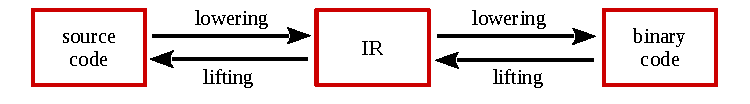
\includegraphics[width=.7\columnwidth]{images/compiler} 
\end{figure}




\newpage

% !TEX root = main.tex

\addtocontents{toc}{\setcounter{tocdepth}{2}}
\section{Notes}

\subsection{Symbolic Execution}

\subsubsection{\cite{K-CACM76} Symbolic execution and program testing} 

\paragraph{Goal}

Test a program using symbols, not actual inputs, which represents a class of inputs (determined by the dependence of the program's control flow on its inputs).

\paragraph{Approach}     
  \begin{itemize}   
    
    \item inputs are seen as symbols ${\alpha}_i$ (integers)
    
    \item execution state:
      \begin{enumerate}
        \item current statement executed
        \item path condition (pc): 
          \begin{itemize}
            \item set of assumptions over inputs made to reach the current statement
            \item initially set to true
          \end{itemize}
      \end{enumerate}

      \item {\tt IF}: when there is a branch: 
        \begin{lstlisting}
      if q
          then ...
          else ...
        \end{lstlisting}
        where q can be any kind of expression over ${\alpha}_i$. Check q, if always false or always true, proceed with
        execution (non forking) and do not alter pc. Otherwise, perform forking by expanding in parallel two branches:
        \begin{enumerate}
          \item pc $\gets$ pc $\wedge$ q (condition satisfied)
          \item pc $\gets$ pc $\wedge$ !q
        \end{enumerate}
        proceed with execution on both branches. pc always remains true.

  \end{itemize}

\subsubsection{\cite{H-TSE77} Symbolic Testing and the DISSECT Symbolic Evaluation System} 

  \paragraph{Goal} 
  Improved symbolic execution engine wrt~\cite{K-CACM76}.

  \paragraph{Approach}

    \begin{itemize}
      \item input commands: if there is a loop with an input instruction (e.g., read) then label the symbol with the path index (index in the execution tree):

        \begin{lstlisting}
      1. for i=1 to N 
      2. x = read(...)
        \end{lstlisting}
      Then:
      \begin{lstlisting}
      x = x:2 (when i=1)
      x = x:4 (i=2)
        \end{lstlisting}

        \item output commands and variable values: problems due to array reference, e.g.:
      \begin{lstlisting}[mathescape=true]
    1. X = array(10)
    2. I = 2
    3. X(I) = 0 $\Rightarrow$ X(I:2) = 0
    4. I = read()
    5. X(I) = 10 $\Rightarrow$ X(I:4) = 10
    6. Y = X(2)
      \end{lstlisting}
      Y is X(2):5 meaning that is the value assigned at the path index 5 or an earlier value assigned to it. To keep track of earlier values, we keep a list of values related to values(X(2)) = \{0, X(2):5\}

      \item users can use some path selection commands to indicate which branches are taken, how many time a loop is executed, add branches, halt

    \end{itemize}

\subsubsection{\cite{KLEE-OSDI08} KLEE: Unassisted and automatic generation of high-coverage tests for complex systems programs} 

\paragraph{Goal}

Symbolic execution engine for generating code coverage tests for C applications.

\paragraph{Approach}

KLEE does not currently support: symbolic floating point, longjmp, threads, and assembly code. Additionally, memory objects are required to have concrete sizes. STP is the constraint solver (see~\cite{EXE-CCS06}).

KLEE works on the LLVM bytecode generate by LLVM-gcc. Given as input the bytecode, it generates inputs (constraints can be put on the number of cmd arguments, their maximum length, maximum times syscall can fail), Tests can be run on actual code, generated with native compiler. Input marked as symbolic have associated a constraint on it (initially this could be nothing). When a conditional is met in the code, a constraint solver determines which branch is taken. If current constraints do not lead to a specific branch, then there is an execution fork. When a bug (exception, memory error) or process exit is hit, the constrain solver is used to obtain valid inputs which lead to that exit point. KLEE analyzes the bytecode and modifies the state based on the side effects given by a statement. If a fork is needed, the state is cloned and a new KLEE process is instantiated. If a load/store works on an address which could point to different objects, for each object a fork is executed and the address is bounded to that object from now on. Memory is not seen as a single array, but divided in many objects (stack, heap objects, etc.) and copy on write is used to minimize overhead due to cloning (e.g., cloning heap has constant cost).

Some aspects:

\begin{itemize}

  \item Process scheduling: Need to decide what is the next KLEE process to run. Different strategies:
    \begin{itemize}
      \item random: a tree is build where internal nodes are branch points, and leaves are the active KLEE processes. A random path is chosen. Notice that all leaves under the same branch point get the same probability to be executed. Properties:
        \begin{enumerate}
          \item avoid starvation (too many forks in one region)
          \item favor nodes high in the tree, which are relatively unconstrained
        \end{enumerate}
      \item uncovered regions: choose process using some heuristics. which can cover uncovered code. Assign weight to each process based on the min distance to uncovered code, consider stack, consider whether that region has recently covered uncovered code. Then pick randomly.
    \end{itemize}
    Each process is executed for time-slice, which is based on the cost of the statement Indeed, expensive instructions should not dominate the execution otherwise limited progress is done.

  \item Query optimization: KLEE spends most of the time querying the constraint solver. Hence, query optimization is crucial. Techniques:
    \begin{itemize}
      \item constraint independence: divide constraints in independent disjoint subsets based on the symbolic variables which they reference. Irrelevant constraints can detected and discarded.
      \item counterexample caching: keep a cache of counterexample based on past queries:
        \begin{itemize}
          \item if a subset of constraints has not solution, any superset does not have as well
          \item if a superset has a solution, any subset has a solution
          \item if a subset has a solution, try it for the superset
        \end{itemize}
    \end{itemize}
  \item Interaction with environment. Invocation to syscalls are replaced with invocations to models. Each model wraps a syscall (e.g., read) and can either just invokes the real syscall or emulated it with a symbolic variant. Whether bind to real or symbolic syscall, it is decided during open() or similar syscall: e.g., if the filename is constant then the actual file is opened, otherwise (i.e., the filename is symbolic) a symbolic file is returned. Notice that:
            \[ \text{open(argv[1])} \]
  will bind to symbolic file and add constraint on argv[1] that specifies that argv[1] is a filename. Notice that a symbolic open() will fail one time and N parallel KLEE processes will be added: one for each possible symbolic file specified by the user (e.g., different sizes, different permissions, they are actual files passed by the user in a specific directory). Hence, N+1 branches are created for a symbolic open(). For efficiency, a symbolic open() will generate only 2 branch: one for covering the fail, and one matching all available symbolic files. Only when needed, this branch is exploded. Notice that syscall failure is covered both for realistic cases (e.g., file not exists) and for uncommon scenarios (e.g., write failure due to no available disk space). Uncommon scenarios can be disabled for efficiency. Notice that when tests are generated, if needed, symbolic files are instantiated using the files specified by the user for the symbolic syscall. Failure of syscall are reproduced during real tests (executed without KLEE) exploiting ptrace.

\end{itemize}

\subsubsection{\cite{EXE-CCS06} EXE: Automatically Generating Inputs of Death} 

\paragraph{Goal}
Identify inputs that may crash an application

\paragraph{Approach}
Custom made constraint solver called STP, available at https://github.com/stp/stp\\


Does not handle floating point values. User must mark all the variable which should be considered as symbolic. CIL is used as source-to-source translator, its output is then compiled with gcc. EXE exploits CIL to propagation of constraints, fork execution if needed,  call STP when execution is finished (e.g., exception, exit, error) and symbols must be instantiated in order to get a valid test. Assertion violations are seen as errors.

Some aspects:
\begin{itemize}
  
  \item STP is a decision procedure for bitvectors and arrays. Instead of using the Nelson-Open's cooperating decision procedures framework, they built STP based on th experience of a previous work called CVCL. Using mathematical and logical identities, constraints are translated in purely propositional logic formulae that are fed to the MiniSAT solver. The code of STP is smaller than CVCL. Data are always seen as untyped. Any operation is mapped to bitvectors. x + y is a bitvector operation, while x + y < z is a formula. Formula are translated in DAGs of single bit operations. 

  \item Each symbolic data is represented as as an array of 8-bit vectors. For each object b of size $|b|$ which is marked as symbolic by the user, EXE create an array $b_{sym}$ of size $|b|$ and track this mapping in a table. Other mappings are added to the table due to an assignment (v = e) or reference to an element of an array (b[e]) (b is imported in STP as an array of the same size).

  \item Construction of an expression e: if there is a read of area of size n, then EXE check if that area is concrete. In this case, the concrete values are inserted in e. Otherwise, e is bind to the concatenation of $b_1,..., b_n-1$. For each distinct byte, if it is concrete, then its value is used. Otherwise, it uses it symbolic expression $(b)_i$. E.g.  $a + i*4$ where a is the starting addr of an array and i an integer of four bytes, then the result is:
    \[ a + (i_sym[3] + i_sym[2] + i_sym[1] + i_sym[0]) * 00...0100 \]

  \item Pointer are seen as array reference at some offset. For this reason, allocation and deallocation are tracked. Double references like **p force to STP concretize *p, fixing a storage location.

  \item Fast array constraints: few translations are needed in order to make STP faster. FTP works on purely functional language:
    \begin{lstlisting}
      // read value v at position i in A
      v  = read(A, i)      
      
      // write on a copy of A, v at A[i]
      A' = write(A, i. v)  
      
      // if condition then a else b
      ite(condition, a, b) 
    \end{lstlisting}
      STP removes any write (note: any write makes sense only if there is a subsequent read):
    \begin{lstlisting}[mathescape=true]
      read(write(A, i, v), j) $\implies$ ite(i == j, v, read(A, j))
    \end{lstlisting}
      STP removes and read, by enforcing that if you read from the same location twice, then you get the same value:
    \begin{lstlisting}
      (read(A, i) = e_1)  and (read(A, j) = e_2)
    \end{lstlisting}
    will be transformed in:
    \begin{lstlisting}[mathescape=true]
      (v_1 = e_1) and (v_2 = e_2) and (i $=$ j $\implies$ v_1 = v_2)
    \end{lstlisting}
  Notice that these techniques increase the size of the formula. For this reason, other optimizations are needed. Array substitution optimization substituting out all constraints of any read(A, c) = e where c is constant:
  \begin{enumerate}
    \item read(A, c) $\implies$ e
    \item ???
  \end{enumerate}
  STP perform lazy evaluation of array refinement: e.g., do not consider some axioms, find solution, see if satisfiable in the original formula then ok, otherwise add some axioms (not all) and then re-evaluate, repeat if needed.

\end{itemize}

\subsubsection{\cite{SAGE-NDSS08} Automated white-box fuzz testing} 

\paragraph{Goal}
Use symbolic execution for performing white-box fuzz testing. This paper is especially important because SAGE (the tool presented in this paper) has been extensively used at Microsoft.

\paragraph{Approach}
Fuzz testing is typically a black-box approach: random inputs are generated and execution is monitored to check errors and unexpected behaviors. Unfortunately, it is unlikely to cover the whole code with random inputs. They propose to exploit symbolic execution to perform fuzz testing.

It works on x86 binaries, exploits Dissolver (a distributed solver), iDNA (to trace execution), and TruScan (to virtually play traces). 

Main aspects:
\begin{itemize}
  \item Generational search: initially starts with a seed input and bound set to zero
    \begin{lstlisting}[mathescape=true]
  check input I for errors (concrete execution, if error than: 
    generate a trace + replay trace for listing executed BB)
  generate symbolic constraints (using the trace)
  childInputs = []
  for (i = bound, i < |constraints|, i++)
    set constraints[bound, ..., i - 1] to true 
      (i.e., exploit concrete input values)
    set constraints[i] to false (possibly this will affect input)
    solve constraints, if SAT:
      create new input I' by updating I
      set bound of I' to I
      add I' to childInputs 
  for each child input, execute (1), compute a score
   based on the number of previously uncovered BBs
  sort child inputs based on score
  for each child input, restart from beginning 
    \end{lstlisting}
    \item SAGE maintains concrete and symbolic states using (value, tag). Tag can be:
      \begin{itemize}
        \item input(m): m-th byte of the input
        \item c: constant
        \item t1 op t2: binary op over two tags: e.g., a concatenation of two tags (e.g., useful to handle registers like cx = (t\_ch, t\_cl))
        \item subtag(t, i): i-th byte of the tag t
      \end{itemize}
    \item Constraint optimizations:
      \begin{itemize}
        \item tag caching
        \item unrelated constraint elimination
        \item local constraint caching
        \item flip count limit
        \item constraint subsumption
      \end{itemize}
\end{itemize}

\subsubsection{\cite{SAB-SP10} All You Ever Wanted to Know About Dynamic Taint Analysis and Forward Symbolic Execution (but might have been afraid to ask)}

This a formalization of symbolic execution and taint analysis.

\subsection{Concolic execution}

Concolic execution has been introduced by~\cite{DART-PLDI05} and later improved by~\cite{CUTE-FSE13}. Notice that concolic execution can be seen a symbolic execution where constraints on the inputs lead to single input instance.

\subsubsection{\cite{DART-PLDI05} DART: directed automated random testing}

\paragraph{Goal}

Automatically generate random tests

\paragraph{Approach}

{\bf Problem:} symbolic execution can hit non linear constraints.\\
{\bf Idea:} do symbolic execution, if needed, perform also concrete evaluation.\\


Three main steps:
\begin{enumerate}
  \item automated extraction of program interfaces. Three kinds of functions:
    \begin{itemize}
      \item program (code)
      \item external functions: routines controlled by the environment and that can be non deterministic. Dart will wrap them and return random results. Assumed that they do not perform any side-effect. Otherwise, they should be simulated.
      \item library functions: not in code, but still deterministic
    \end{itemize}
  \item automatic generation of random tests:. Inputs are generated randomly
  \item dynamic analysis of the program behavior under random testing with automatic generation of new test inputs to direct systematically the execution along alternative program paths
\end{enumerate}

Execution model:
\begin{itemize}
  \item P: the program executed both concretely on random input and symbolically. P execute statements (stored at specific locations $l_i$). which can manipulate the memory.
  \item M: memory (context), a mapping from memory addresses to, for instance, 32-bit words
  \item M' := M + [m -> v]: update of M where M'[m] = v. where m can be an address or a symbolic variable
  \item e: symbolic expression (no side effect!)
    \begin{enumerate}
      \item m: address or symbolic variable)
      \item constant
      \item *(e', e''): multiplication
      \item <=(e', e''): comparison
      \item !(e'): negation
      \item *(e'): deference
    \end{enumerate}
  \item statement at $l_i$:
    \begin{enumerate}
      \item label l: address of another statement
      \item conditional c: if (e) then goto $l_k$
      \item assignment a: m $\gets$ e where m is an address
      \item abort or halt
    \end{enumerate}
  \item evaluate\_concrete(e, M): evaluate e in context M and return a 32-bit value for e
  \item statement\_at(l, M): next statement to be executed at l. If assignment, returns the address where to save the right hand side
  \item input addresses $M_0$: addresses of input parameters for P
  \item input vector I: initial values for values in $M_0$, which gives M (initial context)
  \item A: set of conditional statements
  \item C: set of conditional statements
  \item EXECS := (A u C)* (halt $|$ abort)
  \item program execution w: a finite sequence in EXECS. which can written as:
  
    \[ alpha_1~c_1~alpha_2~c_2~[...]~alpha_{k+1}~s \]
    where:
      \begin{itemize}
        \item $\alpha_i$ in A*
        \item $c_i$ in C
        \item $s \in$ {halt. abort}
      \end{itemize}
      Notice that given I, then w can be determined.
    \item EXECS(P): subset of EXECS valid for P given all possible I. This can be represented as an execution tree, where assignments have one successor, conditionals have one or two successors, leaves are (halt $|$ abort)

\end{itemize}

\subsubsection{\cite{CUTE-FSE13} CUTE: a concolic unit testing engine for C} 

\paragraph{Goal}
Efficiently test code

\paragraph{Approach}

\begin{enumerate}
  \item create a logical input map I that represents all inputs
  \item using I, generates a concrete graph memory for the program
  \item create two symbolic states: one for pointer values and one for primitive values
  \item runs the code on the concrete graph memory, collecting constraints on symbol variables: CUTE finds all the inputs that follows the same path generated by the current concrete inputs
  \item negates constraints to obtain a new logical input map I' which likely can lead to a different path
  \item repeat from (1) using I'
\end{enumerate}


Notice that when a constrain cannot be solve, the concrete value is considered. If due to this, some paths cannot be explored (the concrete value always lead to the same branch) then a new execution of CUTE is started where other random inputs are used as concrete values.

Notice that if a functions takes as input a data structure then two approached can used:
\begin{itemize}
  \item exploit a chain of calls for initializing the data structure
  \item exploit data structure invariants specified by the user through few notations
\end{itemize}

Simple constraints are set on pointer:
\begin{enumerate}
  \item equal or not equal to another pointer
  \item NULL or not NULL
\end{enumerate}

\subsection{Applications}

\subsubsection{\cite{FIRMALICE-NDSS15} Firmalice - Automatic Detection of Authentication Bypass Vulnerabilities in Binary Firmware} 

\paragraph{Goal}
Analyze a firmware and detect auth bypass inside it.

\paragraph{Approach}

Steps:
\begin{enumerate}
  \item Firmware loading: 
    \begin{itemize}
      \item disassembly: they assume that the blobs are not excessively obfuscated or ciphered. If they are then [KRV-USENIX-SEC15]
      \item base address determination: analyze jump table (referred by indirect jumps)
      \item entry point discovery: build call graph, consider root nodes of weakly connected components
    \end{itemize}
  \item Security policies: user should define when bypass occurs e.g., if code reach auth success string, actions (read by a device), reserved memory areas, privileged code
  \item Static program analysis:
    \begin{itemize}
      \item build context sensitive CFG exploiting a symbolic execution engine for resolving jumps
      \item build control dependency graph (CDG), obtained by transforming CFG
      \item build data dependency graph (DDG) that shows how instructions correlate wit each other with respect to the production and consumption of data. Obtained by using data flow analysis approach in [TG-CC06]
      \item backward slicing: given a program point produce every statement on which that point depends. Slicing technique from [KJL-SCAM03]. Creation of authentication slice (analyze all code is costly).
    \end{itemize}
  \item Symbolic exec engine to find inputs to reach privileged code. Concepts from~\cite{KLEE-OSDI08} [FUZZBALL-SSTA11] \cite{MAYHEM-SP12}.
    \begin{itemize}
      \item used Z3 as constraint solver
      \item symbolic summaries: instead of analyzing all subroutines, tries to model common routines (e.g., libc) and detect them in blobs. Several test cases that check pre/post conditions.
      \item lazy initialization: if there is a read over uninitialized data, then identify writes to that area, analyze path with and without initialization
    \end{itemize}
  \item  Authentication bypass check: analyze inputs that reach s code, if not concrete generate a function that can generate them. Also identify data exposed.
\end{enumerate}

\subsubsection{\cite{MAYHEM-SP12} Unleashing MAYHEM on Binary Code} 

\paragraph{Goal}
Automatically generate exploit for a binary.

\paragraph{Approach}      
MAYHEM has two core parallel components:
\begin{enumerate}
  \item CEC: concrete execution client
  \item SES: symbolic execution server
\end{enumerate}

Steps:
\begin{enumerate}
  \item users specify class of input parameters
  \item CEC loads the binary, instruments the code, and performs dynamic taint analysis, detecting for each block of instruction, which are tainted and have impact on the flow (cjmp or call). When this is detected by CEC, the execution is suspended and block is sent to the SES
  \item Instructions are translated by the SES into an intermediate language using [BAP-CAV11] and keep track of concrete values (provided by CEC). SES maintains two kinds of formula:
  \begin{itemize}
    \item path formula: condition on symbols that lead to the current path
    \item exploitable formula: it determines if the attacker is able to:
    \begin{itemize}
      \item modify EIP
      \item execute a payload
    \end{itemize}
  \end{itemize}
  If needed the SES forks execution and the informs CEC the branch where continue the concrete execution. If the resources cap is reached, then, instead of actually forking, a checkpoint is created. A checkpoint is a way to save partial state (only symbolic state is saved, not concrete) to disk and restore it when resources are available. To restore concrete execution, the symbolic state is exploited (e.g., choose input values).Copy on write is used to take snapshots efficiently.
  \item if there is a tainted jump then MAYHEM builds an exploitable formula and uses the solver to check whether it is satisfiable. If exploit found, then the goal is reached. Otherwise, explore other paths.
\end{enumerate}

Other aspects:
\begin{itemize}
  \item A virtualization layer is needed to isolate different concrete executions and hide their side effects
  \item MAYHEM uses precondition symbolic executions, hints by user which restricts the solution space for symbols and thus help the symbolic execution engine.
  \item MEYHEM uses an index-based memory model:
    \begin{itemize}
      \item $\pi : I \to E$ where i is a 32-bit index in I, e is an expression in E 
      \item $e \gets load(\pi, i)$ where i indexes memory $\pi$, e represents the contents of the i-th memory cell
      \item $store(\pi, i, e)$: a new memory is returned
    \end{itemize}
    Unfortunately, fully symbolic memory is not scalable. Concretizing any memory operations is too limiting in practice. For this reason, MAYHEM models memory partially:
    \begin{itemize}
      \item writes are always concretize
      \item reads are allowed to be modeled symbolically
    \end{itemize}
    To make this efficient, several techniques are adopted: 
    \begin{itemize}
      \item upper and lower bounds on reference
      \item value set analysis
      \item refinement cache
      \item lemma cache
      \item index search trees
      \item bucketization with linear function
    \end{itemize}
    If a memory object is too big, then an index pointing to it will be concretized.
  \item exploits generated by MAYHEM are: buffer overflows, format string attacks
\end{itemize}

\subsubsection{\cite{AEG-NDSS11} AEG: Automatic Exploit Generation} 

\paragraph{Goal}
Automatically generate exploits.

\paragraph{Approach}

Mixed approach: 
\begin{itemize}
  \item source code analysis to improve scalability (in practice LLVM bytecode is used)
  \item binary and runtime information to exploit programs
\end{itemize}

To make symbolic execution feasible, they propose two techniques:
\begin{itemize}
  \item preconditional symbolic execution
  \item path prioritization
\end{itemize}

They first execute a program symbolically. If they detect a bug (e.g., out of bounds), then it concretize an input for that bug. Using dynamic analysis, memory layout and the stack is analyzed in order to determine additional constraints needed for obtaining a valid exploit (e.g., where to put the shell code). The solver builds the input containing the exploit (return to stack or return to libc).\\

Some aspects:
\begin{itemize}
  \item Preconditionale symbolic execution: a way of restricting symbolic execution to only specific branched by imposing additional constraints. This may make symbolic execution unsound if the preconditions are excessively restrict. In general, preconditions should allow AEG to find at least one solution (i.e., exploit). AEG may add the following preconditions:
  \begin{itemize}
    \item none
    \item known length: inputs are known to have a specific maximum size. E.g., if input is a string, then each byte up to the length is different from \textbackslash0, while the last one is \textbackslash0. Low impact on space solution, but it helps with strcpy and other buffer overflow vulnerable functions.
    \item known prefix: inputs are known to have a specific prefix. E.g., a http server will see input containing GET header. May have a huge impact on solution space.
    \item concolic execution: use the value from a concrete execution. This is useful when an input is known to crash the application and AEG is used to obtain an exploit. Only one input.
  \end{itemize}
  \item Path Prioritization: heuristics
    \begin{itemize}
      \item buggy-path first: give priority to path where errors have been seen even if they were not exploitable
      \item loop exhaustion: try to exhaust loops, this should make emerge buffer overflows. To avoid starvation:
        \begin{itemize}
          \item use preconditions to bound iterations
          \item allow only one executor to perform loop exhaustion
        \end{itemize}
    \end{itemize}
  \item Environment modeling:
  \begin{itemize}
    \item symbolic files: similar to KLEE
    \item symbolic sockets: AEG has model for several network syscalls
    \item environment variables: support for get\_env
    \item syscall: models for most common syscalls
  \end{itemize}
\end{itemize}


\subsubsection{\cite{KKM-USEC05} Automating mimicry attacks using static binary analysis} 

\paragraph{Goal}
Evade IDS with mimicry attacks (use a benign sequence of system calls but for malicious purposes).

\paragraph{Approach}
Modern IDS may control the instruction address of the syscall invoker and detect if the control flow is altered (the check is done before and after the syscall). However, this is not enough if the attacker can perform multiple distinct attacks (i.e., regain control multiple times) or modify memory used by syscall (e.g., modify args of execve). \\

Some aspects:
\begin{itemize}
  \item Execution state: state S of program p as a snapshot of the content of processor registers and all valid memory locations. Initially, a symbol is introduced for each register and for each location in a writable memory segments. A new symbol is introduced whenever a new location is read. FP is not supported. A special symbol (bottom) is used whenever no information is available on a memory location (but it is known during a concrete execution). Constraint of symbols are limited to linear expression. Loop or conditional branches add constraints to the path constraints (e.g., L=0 or L>=0 for loops, condition or !condition for branches) and lead to forks. In order to avoid starvation, number of iterations for a loop are approximated using few static techniques, which however may harm precision. To analyze the effect of a loop, fixpoints are introduced.
  \item A fixpoint F is an approximation of the effect of loop body on an execution state. F approximates the state after the execution of loop whenever the initial state before the loop was F. TRansforming an execution state to a fixpoint state is defined as widening. Construction of the fixpoint:
  \begin{itemize}
    \item S1: state after first iteration
    \item S2: state after second iteration
    \item compare S1 and S2: assign bottom to each symbol that has been altered
    \item repeat until there is no difference between Si and Si+1
    \item if there is a branch inside the loop, then either the branch is known or its condition is on a symbol which has been assign to bottom. In this case, two parallel states are created and then compared.
  \end{itemize}
  \item Generate a configuration for a mimicry:
  \begin{itemize}
    \item indirect jump: add constraints that:
      \begin{itemize}
        \item address s\_t (used by the indirect jmp) has to be equal to the target t (malicious code)
        \item indirect jump is executed.
      \end{itemize}
    \item data transfer: add constraints that:
      \begin{itemize}
        \item source is t
        \item destination is a return address 
        \item no system call is invoked between modification of return address and its use (otherwise it will be detected by an IDS)
      \end{itemize}
  \end{itemize}
  \item They assume that different symbolic expression refer to different memory locations. This is optimistic but it is needed to avoid complex pointer alias analysis. They perform a posteriori check.

\end{itemize}

\subsubsection{\cite{FUZZBALL-ESORICS13} HI-CFG: Construction by Binary Analysis, and Application to Attack Polymorphism} 

\paragraph{Goal}
Find the input that has lead to generate a specific output. HI-CFG is a data structure used by Fuzzball (symbolic engine) described in a technical report entitled {\em Transformation-Aware Symbolic Execution for System Test Generation}.

\paragraph{Approach}
They propose a symbolic approach which exploit knowledge of the transformations applied to the input data. A key idea is to analyze multiple transformations in a pipeline separately one by one (starting from the last one). E.g.:

\[y = F(G(x)) \text{ where y is an output} \]

FuzzBall first finds x' such that y = F(x'), then x such that x' = G(x). Transformations are described by the HI-CFG data structure, which can be build by dynamically analyzing a binary (using a benign input), and that contains CFG + information flow + data flow.

They assume that y can be obtained in some way and thus is a valid output. In particular, they focus on transformations that are:
\begin{itemize}
  \item surjective: every element of the co-domain is mapped to by at least one element of the domain
  \item sequential: when a byte of the output is written, then it is final
  \item streaming: a pipeline that start generating output before seeing the whole input
\end{itemize}

FuzzBall explore one path at time, never in parallel. If there is branch, a choice is made to decide where to continue. When execution is finished, it tries another branch. To reduce solution space:
\begin{itemize}
  \item search pruning: prune prefixes of the input buffer contents that produce the wrong prefix of the output buffer contents
  \item search prioritization: prioritize path that have produced the larger amount of the output. Use this criteria 0.95\% of the times, otherwise starvation is possible.
\end{itemize}

Symbolic array accesses array[i] where i is symbolic. Two approaches:
\begin{itemize}
  \item multi-way branch: for each possible value of i, start a new execution. Many execution, but symbolic formula are simple (i is concrete).
  \item large formula: put constraints on i in the formula (i = 0 or i = 1 or ...). Few executions, but complex formula.
\end{itemize}

\subsubsection{\cite{CFB-ACSAC06} Static Detection of Vulnerabilities in x86 Executables} 

\paragraph{Goal}
Find vulnerabilities in x86 binaries.

\paragraph{Approach}
Not complete nor sound due to imprecision in handling of loops, x86 modeling and libc modeling.
Implementation built on top of \cite{KKM-USEC05}.

\begin{itemize}
  \item Preliminaries steps:
    \begin{enumerate}
      \item binary is disassembled using the basic linear-sweep algorithm
      \item few heuristics to resolve indirect call and jump. This is needed for building CFG.
        \begin{itemize}
          \item backtrack in code to determine base location of jump table and its size. This compiler-specific.
          \item inter-procedural constant propagation by symbolically executing some functions to determine a set of possible targets
          \item similar approach for derive return function pointers
        \end{itemize}
      \item detection of loops and recursive function calls:
        \begin{itemize}
          \item loops: approach described in {\em Identifying loops using dj graphs}
          \item recursive functions: topological sort algorithm on CFG
        \end{itemize}
      \item resolve library functions through analysis of PLT and relocation table
    \end{enumerate}
\end{itemize}

Some aspects:
\begin{itemize}
  \item Symbolic execution:
    \begin{itemize}
      \item effects of x86 instructions have been modeled
      \item symbols are introduced whenever reading from registers or locations that do not have a concrete value or due to library functions which interact with the environment
      \item values are seen as integers
      \item all effects which produce non-linear constraints return an unknown symbol (i.e., bottom)
      \item solver is Parma Polyhedra Library
      \item loops are handled in two ways:
        \begin{itemize}
          \item if termination condition can statically determined then full analysis
          \item otherwise at most three iterations: if more than three an approximation of the state is computed
        \end{itemize}
      \item recursive function calls terminate immediately: recursive loops explored only one
      \item alias analysis: not done, optimistic approach that each expressions refer to different locations
    \end{itemize}
  \item Vulnerabilities analysis: They check for insecure uses of popen() and system(). This is done using taint analysis:
    \begin{itemize}
      \item identification of untrusted sources
      \item propagation of tainted data
      \item generation of alerts when tainted data reaches a sensitive sink (popen or system)
    \end{itemize}
    Taint analysis is done using symbolic execution. Since the main interest is around sinks, program slicing is applied to optimize symbolic execution. This is done by looking at the CFG but this is likely to be imprecise.
  \item Several libc functions have been modeled to capture external sources of taint data.
\end{itemize} 

\subsubsection{\cite{BNS-SP06} Towards Automatic Generation of Vulnerability-Based Signatures} 

\paragraph{Goal}
Create vulnerability-based signature which are robust to polymorphism and metamorphism (different syntax, same semantic).

\paragraph{Approach}
The main idea is to construct a signature based on the vulnerability and not based on an exploit. 

Aspects:
\begin{itemize}
  \item Given a known exploit, they assume that a third-party analysis can provide:
    \begin{itemize}
      \item P: a binary (the program)
      \item x: exploit string
      \item T: execution trace of P over x
      \item c: vulnerability condition
    \end{itemize}
    The vulnerability is (P, c), the execution trace can be seen as T(P, x). If T satisfied c then T $\models$ c.
    The goal is to automatically detect other x' which tries to exploit c. Formally: $L_{P, c}$ is the set of all inputs x such that T(P, x) $\models$ c. Their approach builds a function MATCH that is able to detect any x in $L_{P, c}$. The condition is a function that return true if an unsafe instruction is executed. They assume that c is provided: e.g., an algorithm that check safe pointers.
  \item Three language classes can be used to represent $L_{P,c}$:
    \begin{itemize}
      \item turing machine signatures: sound but potentially time unbound. For instance, one could write a program which simulate P and check for the vulnerability condition
      \item symbolic constraint signature: the main idea is to use a set of boolean formulas which approximate the turing machine signature. There are no loops when evaluating a symbolic constraint signature. If there is loop in the program and it cannot be statically inferred how many times to unroll it, upper or lower bound must be provided.
      \item regular expression signatures: least powerful 
    \end{itemize}
  \item Few definitions:
    \begin{itemize}
      \item MEP: monomorphic execution path, a single execution path that reaches the vulnerability point
      \item PEP: polymorphic execution path, all execution paths that reach the vulnerability point
      \item chop: all the instructions execution between a read (point where exploit may be read) and the the vulnerability point
    \end{itemize}
  \item Steps:
    \begin{itemize}
      \item identify function boundaries of the binary, then translate it into IR
      \item compute the chop given a trace T: they use a previous work that analyze the CFG. The chop is not precise since they do not perform pointer analysis. The main idea is to perform a reachability analysis. Indirect jumps are problematic.
      \item compute the signature:
        \begin{itemize}
          \item TM signature:
            \begin{enumerate}
              \item MEP TM signature:
              take the IR instructions and based on the trace mark branches: if they take another path than the one of the trace then mark them as benign flag. If vulnerability point is reached then it returns exploit flag.
              \item PEP TM signature: similar to MEP signature but use chop instead of the trace
            \end{enumerate}
          \item Symbolic constraint signature: they build this signature by symbolically executing on the TM signature (MEP or PEP, respectively). Required to convert IR in SSA form. The PEP signature is imprecise since loops need to be evaluated: they are handled by computing fixed points
          \item Regular expression signatures: built on top of symbolic constraint signatures by building a language that is consisted with symbolic constraints
        \end{itemize}
    \end{itemize}
\end{itemize}

\subsubsection{\cite{MineSweeper-BOTNET08} Automatically Identifying Trigger-based Behavior in Malware} 

\paragraph{Goal}
Detect malware that perform malicious actions only under specific conditions (triggers).

\paragraph{Approach}
They work on binaries, which can be packed.\\

Steps:
\begin{enumerate}
  \item users selects kinds of trigger events (e.g., calls to some system libraries related to time, network, etc.). Pre-defined lists or custom based. Minesweeper can execute malware and observe which system calls are used. This can help the user choose trigger events.
  \item The program is executed: trigger events are associated to symbols, other things get concrete values. Basically, it's a form of concolic execution. Solver returns the values for trigger events which make execution explore additional paths.
    \begin{itemize}
      \item loads and stores are symbolically executed using lambda abstractions: see Types and Programming Languages, MIT PRESS
      \item reads and writes from symbolic addresses are challenging. In practice, they are rare since only few symbols associated to trigger events.
      \item the solver may not be able to solve a formula within a short amount of time: they give up on that path. An alternative is to optimistically follow the path where the branch is true. Common scenario: check that an hash is equal to a value, if algorithm is robust then it is unlikely that the solver could solve the constraints. Sometimes it could be useful to give information about unsolved formulas to the user.
      \item STP as solver
      \item execution forks is emulated as multiple distinct executions
      \item they use QEMU
    \end{itemize}
  \item Values returned by the solver are used to fully execute the malware and observe the trigger-based behavior
  \item A control flow graph is visually shown to the user in order to help him understand the impact of trigger events
\end{enumerate}

\subsubsection{\cite{SLG-NDSS08} Impeding Malware Analysis Using Conditional Code Obfuscation} 

\paragraph{Goal}
They demonstrate how system that symbolically execute malware to detect trigger events can be harmed.

\paragraph{Approach}
For each branch, make the decision based on the comparison with the result of a robust hash function. Inside the branch, decrypt the code that should be executed afterwards.

\subsubsection{\cite{MKK-SP07} Exploring Multiple Execution Paths for Malware Analysis} 

Very similar to \cite{MineSweeper-BOTNET08}. Differences:
\begin{itemize}
  \item QEMU with guest OS Windows 2000
  \item Kinds of trigger events are detected using dynamic analysis (tracing library routines, system calls, etc.)
  \item they analyze execution: when there is branch they follow it. Later they restore the state and follow another branch.
  \item symbolic constraints can be solved only if linear.
\end{itemize}

\subsubsection{\cite{ANGR-SP16} State of) The Art of War: Offensive Techniques in Binary Analysis} 

Security -- Static analysis techniques:
\begin{itemize}
  \item recovering the control flow graph: main problem is given by indirect jumps, which can be computed at runtime, context-sensitive (e.g., invocation of a user callback), object-sensitive invocations (e.g., virtual functions). In practice, many techniques are used to deal with indirect jumps, however soundness and completeness of the CFG can be significantly affected by them.
  \item discovering graph-based vulnerability: a bug can be modeled as a set of nodes in a control flow graph (or data flow, or control-dependence).
  \item value-set analysis: this analysis attempts to find a tight over approximation of the program state (values and registers). It can be used track indirects jumps. It may lack accuracy but is sound. It can be used to identify overlapping buffers, problem that can lead to buffer overflows.
\end{itemize}

Security -- Dynamic analysis techniques:
\begin{itemize}
  \item fuzzing: start from a random input, mutate it, test code to find bugs:
    \begin{itemize}
      \item coverage-based fuzzing: use coverage metric to decide where it should continue to test
      \item taint-based fuzzing: analysis of how the user input flows through code and based on this generate different inputs
    \end{itemize}
  \item dynamic symbolic execution (concolic execution): subset of symbolic execution. While the system emulates the program execution, it tracks symbol constraints, then negates constraints to explore other branches. Main problem is path explosion.
    \begin{itemize}
      \item symbolic-assisted (guided) fuzzing: exploit symbolic execution to make progress when fuzzer tools get stuck.
      \item under-constrained symbolic execution: analyze symbolically parts of the application. This can give false positives, since the context may never shows some bugs of some piece of code.
    \end{itemize}
\end{itemize}

Notice that techniques such as de-randomization can generate crashing inputs which are not actually replayable. AT the end, the only way to find a real bug is to run it in the real environment.

{\tt angr} is cross-platform, cross architecture. It supports different analysis paradigms: need to support different memory models. Using {\tt angr}, several results from previous papers (e.g., \cite{AEG-NDSS11}), not only related to symbolic execution,  can be easily reproduced. It is composed by several submodules:

\begin{itemize}
  \item {\em intermediate representation}: VEX and PyVEX.
  \item {\em binary loading}: loader called {\tt CLE (CLE Loads Everything)} that exploits several native libraries (e.g., {\tt elftools}, {\tt pefile}) to support many formats.
  \item {\em program state representation/modification}: {\tt SimuVEX} simulates the state:
    \begin{itemize}
      \item registers
      \item symbolic memory: index-based memory similar to~\cite{MAYHEM-SP12}
      \item abstract memory: a region-based memory, typically used by most static analysis tools
      \item POSIX: track state of files
      \item log: it keeps a log of any side-effect on the state
      \item inspection: it can easily debugged, allowing breakpoints, taint conditions, symbolic conditions, instrumentation (e.g., memory accesses).
      \item solver: {\tt claripy}
      \item architecture info: a way to expose properties of the architecture (e.g., word size).
    \end{itemize}  
  \item data model: it exploits {\tt claripy} to write expression trees over values. Several backends/frontends: e.g.,~\cite{Z3-TACS08}, VSA~\cite{WYSINWYX-TOPLAS10}.
  \item full-program analysis: {\tt PathGroup} tracks paths as they run through an application which is useful to implement path prioritization, {\tt Analysis} manages the life-cycle of static analysis (e.g., CFG recovery).
\end{itemize}

\paragraph{CFG recovery} Two algorithms:
\begin{itemize}
  \item {\tt CFGAccurate}: slow, iterative CFG recovery, mix of {\em force execution}, {\em backwards slicing}, {\em symbolic execution} to recover indirect jumps. It computes a {\em backward slicing} from unresolved jumps and then ue the constraint engine to identify possible targets.
  \item {\tt CFGFast}: fast but inaccurate, the goal is to get quickly high coverage, based on a dissambler. Performs several steps: function identification,  recursive dissasembly, indirect jump resolution (through light-weighted alias analysis, data flow-tracking, heuristics).
\end{itemize}

\paragraph{Value Set Analysis} Static technique that combines numerical analysis and pointer analysis. It uses an abstract domain to approximate values of location and of registers may hold at each program point. VSA analyzes a program until it reaches a {\em fix point} for all program points in the function: e.g., it returns a complete lists of all possible write target given a write operation. To make it VSA effective: discrete set of strided intervals, applying an algebreic solver to path predicates, adopting a signedness-agnostic domain.

\paragraph{Dynamic Symbolic Execution} Same approach as~\cite{MAYHEM-SP12}, it uses~\cite{Z3-TACS08}. State merging is done using approach presented in~\cite{VERITESTING-ICSE14}.

\paragraph{Under-Constrained Symbolic Execution} Same approach as in~\cite{RE-USEC15}. The main idea is to symbolically execute each function separately. The main issue is that is not replayable, since it lacks its {\em context}. For this reason, the missing context is tagged as under-constrained. Improvements: global memory is treated as under-constrained, additional path limiters, false positive filtering.

\paragraph{Symbolic-Assisted Fuzzing} They have developed~ \cite{DRILLER-NDSS16}.

\paragraph{Crash reproduction} Similar approach presented by~\cite{REPLAYER-CCS06}. Given a program $P$, an initial state $s_a$, crash state $q_a$, input $i_a$ that brings from $s_a$ to $q_a$: sometimes $i_a$ cannot be reproduced (e.g., it works only in a de-randomized execution). Using symbolic execution, they obtain the full input $i_b$ that can be used to replay the crash. 

\paragraph{Exploit generation and hardening} Similar approach as~\cite{AEG-NDSS11,MAYHEM-SP12}. For hardening, they use a ROP compiler.


\subsubsection{\cite{DRILLER-NDSS16} Driller: Augmenting Fuzzing Through Selective Symbolic Execution}

\paragraph{Goal} Find bugs in code.

\paragraph{Approach} Interleaved use of a fuzzing technique and symbolic execution. The main idea is that fuzzing techniques are fast and effective at exploring a {\em compartment} of a program but they straggle at exploring other {\em compartments}. Strategy: use as much as possible the fuzzer, when it gets stuck, switch temporarily to concolic execution. Their fuzzer is based on {\em American Fuzzy Loop (AFL)}.


\begin{comment}

\subsubsection{\cite{}} 

\paragraph{Goal}
\paragraph{Approach}

\begin{itemize}
  \item test
\end{itemize}

\begin{enumerate}
  \item test
\end{enumerate}

\begin{lstlisting}
\end{lstlisting}

\end{comment}

\subsection{Other interesting papers}

\subsubsection{Methodology}
A list of papers about symbolic execution (methodology) that we are currently reading:
\begin{itemize}
  \item \cite{BCE-TACAS08} RWset: Attacking Path Explosion in Constraint-Based Test Generation
  \item \cite{CKC-TOCS12} The S2E Platform: Design, Implementation, and Applications
  \item \cite{BPS-SPE00} A static analyzer for finding dynamic programming errors
  \item \cite{KCF-PLDI10} Mixing type checking and symbolic execution
  \item \cite{KPV-TACAS03} Generalized Symbolic Execution for Model Checking and Testing
  \item \cite{BLISS-TSE15} BLISS: Improved Symbolic Execution by Bounded Lazy Initialization with SAT Support
  \item \cite{GDV-ISSTA12} Probabilistic symbolic execution
  \item \cite{CGK-ICSE11} Symbolic execution for software testing in practice: preliminary assessment
  \item \cite{PRV-ISSTA11} Symbolic execution with mixed concrete-symbolic solving
  \item (EMILIO) \cite{DRILLER-NDSS16} Driller: Augmenting Fuzzing Through Selective Symbolic Execution 
  \item \cite{KKB-PLDI12} Effient State Merging in Symbolic Execution
  \item \cite{SPM-ISSTA09} Loop-Extended Symbolic Execution on Binary Programs
  \item \cite{CWD-SSP15} Program-Adaptive Mutational Fuzzing
  \item (EMILIO) \cite{ED-ISSTA07} Under-constrained Execution: Making Automatic Code Destruction Easy and Scalable
  \item (EMILIO) \cite{VERITESTING-ICSE14} Enhancing symbolic execution with veritesting
  \item (EMILIO) \cite{RE-USEC15} Under-Constrained Symbolic Execution: Correctness Checking for Real Code
  \item (EMILIO) \cite{CS-CACM13} Symbolic execution for software testing: three decades later
  \item \cite{PATHFINDER-ASE10} Symbolic PathFinder: Symbolic Execution of Java Bytecode
\end{itemize}

\subsubsection{Applications}
A list of papers about applications of symbolic execution that we are currently reading:
\begin{itemize}
  \item \cite{LOOP-CCS15} LOOP: Logic-Oriented Opaque Predicate Detection in Obfuscated Binary Code
  \item \cite{BDG-CCS14} Automating Information Flow Analysis of Low Level Code
  \item \cite{ZFM-CCS13} Obfuscation resilient binary code reuse through trace-oriented programming
  \item \cite{BC-CCS14} A Computationally Complete Symbolic Attacker for Equivalence Properties
  \item \cite{MWX-USEC15} TaintPipe: Pipelined Symbolic Taint Analysis
  \item \cite{BLR-WOOT15} Symbolic Execution for {BIOS} Security
  \item \cite{CJS-SP05} Semantics-Aware Malware Detection
  \item \cite{KRV-ACSAC04} Detecting Kernel-Level Rootkits Through Binary Analysis
  \item \cite{YD-CCS15} Symbolic Execution of Obfuscated Code
  \item \cite{CWO-ASPLOS06} Temporal search: detecting hidden malware timebombs with virtual machines
  \item \cite{BHK-TR07} BitScope: Automatically Dissecting Malicious Binaries
  \item (EMILIO) \cite{ANGR-SP16} (State of) The Art of War: Offensive Techniques in Binary Analysis
  \item \cite{CRAX-SERE12} CRAX: Software Crash Analysis for Automatic Exploit Generation by Modeling Attacks as Symbolic Continuations
  \item \cite{REPLAYER-CCS06} Replayer: automatic protocol replay by binary analysis
\end{itemize}

\bibliographystyle{abstract} %abbrv
\bibliography{symbolic}

\end{document}